\chapter{Supplemental}
%\counterwithin{figure}{section}
%\beginsupplement


\begin{figure}[H]
\centering
    % /Users/janet/Dropbox/thesis/tex/chapter1/figures/supplemental/FigureS1.png
     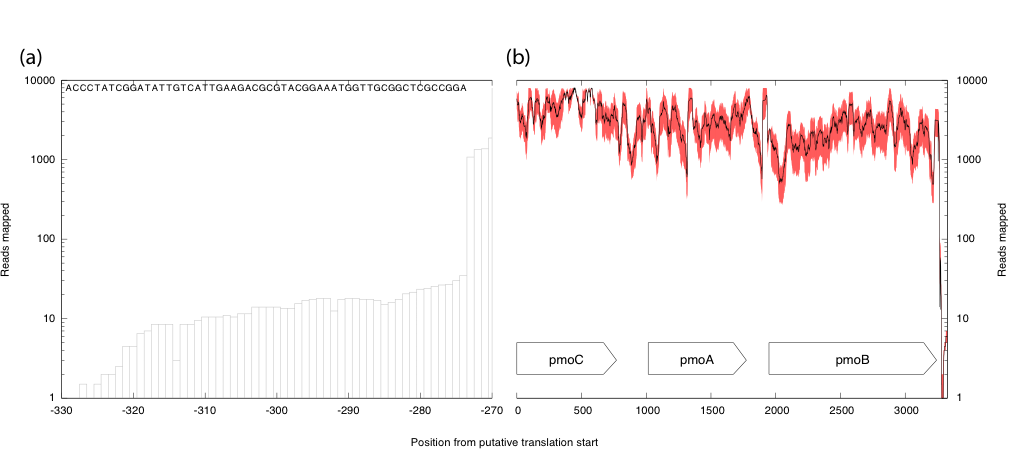
\includegraphics[width=1.0\textwidth]{./tex/chapter1/figures/supplemental/FigureS1.png}
     \begin{singlespace}
     \caption[RNA-Seq reads mapped per base relative to start of \textit{pmo}-operon.]{
        RNA-Seq reads mapped per base relative to start of \textit{pmo}-operon.
        Left, the average number of reads mapped to the region -330 to -270 upstream from the start of \textit{pmoC} for two biological replicates.
        The sequence at each base is shown above the bars.
        Right, the range (shown in red) and mean of two biological replicates (shown as black line) for the number of reads mapped per base for the coding and downstream region of the \textit{pmo}-operon.}
     \label{fig:S1} % label before \end{singlespace} or references break.
     \end{singlespace}
\end{figure}

\begin{figure}[H]
\centering
     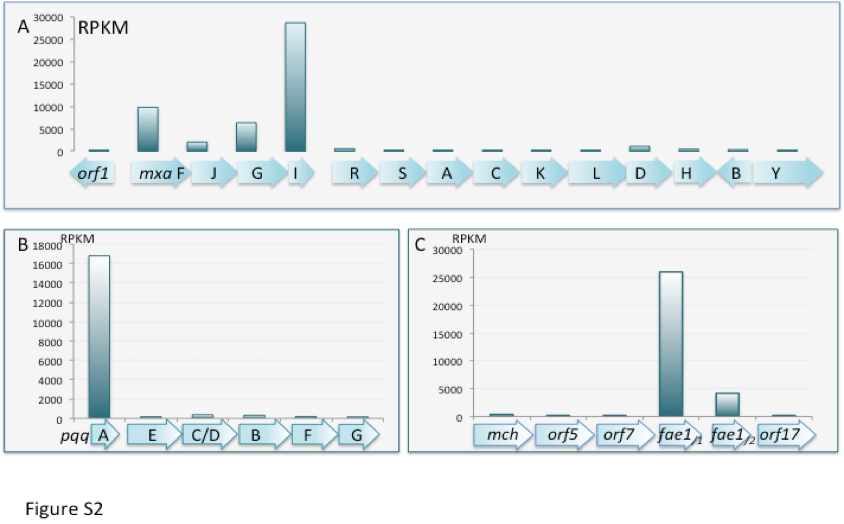
\includegraphics[width=1.0\textwidth]{./tex/chapter1/figures/supplemental/FigureS2.png}
     \begin{singlespace}
     \caption[Genetic organization and relative expression (RPKM) of the \textit{mxa} gene cluster.]{
        Genetic organization and relative expression (RPKM) of the \textit{mxa} gene cluster (A), the \textit{pqq} gene cluster (B) and cluster of genes encoding reactions of the H$_4$MPT-linked C1 transfer pathway (C).}
     \label{fig:S2} % label before \end{singlespace} or references break.
     \end{singlespace}
\end{figure}

\begin{figure}[H]
\centering
     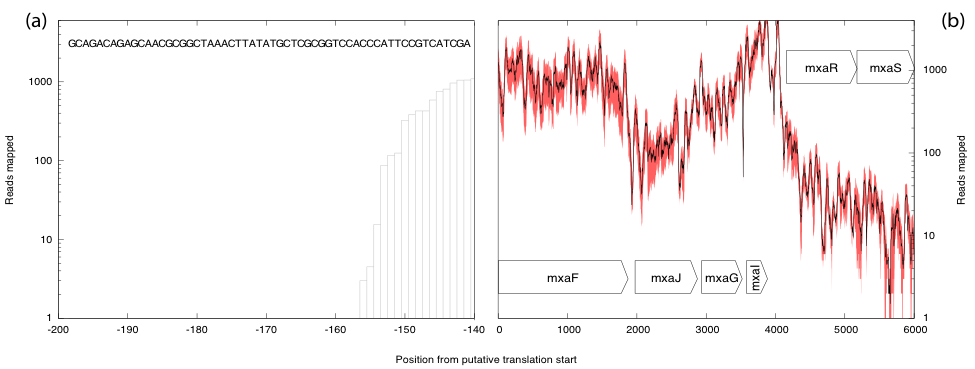
\includegraphics[width=1.0\textwidth]{./tex/chapter1/figures/supplemental/FigureS3.png}
     \begin{singlespace}
     \caption[RNA-Seq reads mapped per base relative to start of \textit{mxaF} ORF]{
        RNA-Seq reads mapped per base relative to start of \textit{mxaF} ORF.
        Left, the average number of reads mapped to the region -200 to -140 upstream from the start of \textit{mxaF} for two biological replicates.
        The sequence at each base is shown above the bars.
        Right, the range (shown in red) and mean of two biological replicates (shown as black line) for the number of reads mapped per base for the coding and downstream region of the \textit{mxaF} cluster.
        }
     \label{fig:S3} % label before \end{singlespace} or references break.
     \end{singlespace}
\end{figure}

\begin{figure}[H]
\centering
     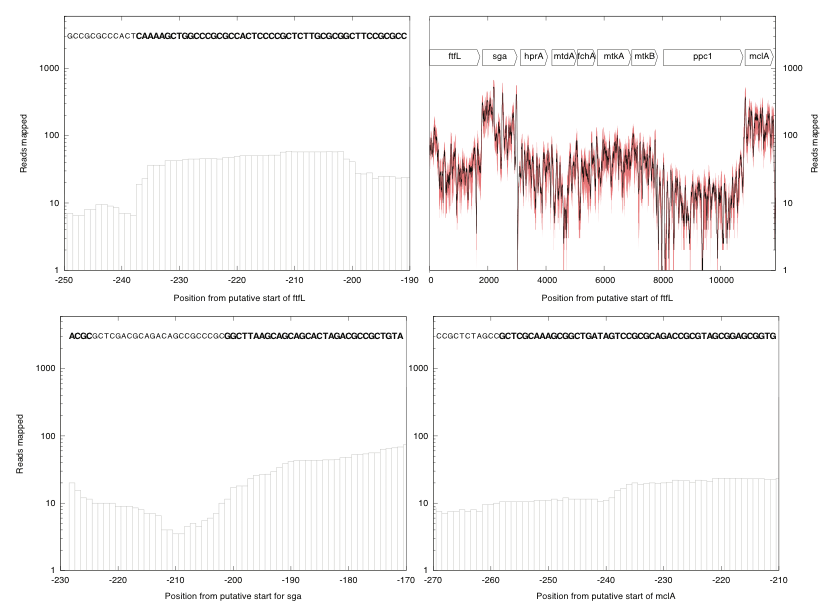
\includegraphics[width=1.0\textwidth]{./tex/chapter1/figures/supplemental/FigureS4.png}
     \begin{singlespace}
     \caption[RNA-Seq reads mapped per base relative to start of serine cycle gene operon.]{
        RNA-Seq reads mapped per base relative to start of serine cycle gene operon.
        The log10 average number of reads mapped at each base from biological replicates one and two is shown.
        In (A), the upstream location spanning -250 to -190 from putative start of \textit{ftfL}.
        (B) The expression over the entire operon.
        Note the several drop to near zero upstream indicating the operon is not co-transcribed.
        (C) The -230 to -170 region upstream from \textit{sga}.
        Bases from the +strand are shown across the top of the figure.
        (D) The -270 to -210 region upstream of \textit{mclA}.
        }
     \label{fig:S4} % label before \end{singlespace} or references break.
     \end{singlespace}
\end{figure}


\begin{figure}[H]
\centering
     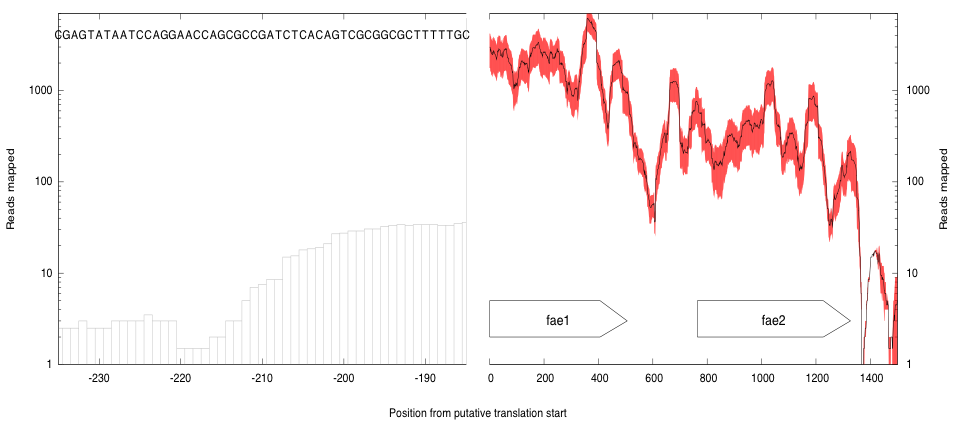
\includegraphics[width=1.0\textwidth]{./tex/chapter1/figures/supplemental/FigureS5.png}
     \begin{singlespace}
     \caption[RNA-Seq reads mapped per base relative to start of \textit{fae1-1}.]{
        RNA-Seq reads mapped per base relative to start of \textit{fae1-1}.
        Left, the average number of reads mapped to the region -235 to -185 upstream from the start of \textit{fae1-1} gene for two biological replicates.
        The sequence at each base is shown above the bars.
        Right, the range (shown in red) and mean of two biological replicates (shown as black line) for the number of reads mapped per base for the coding and downstream region
            of the \textit{fae1-1} and \textit{fae1-2} genes.
        }
     \label{fig:S5} % label before \end{singlespace} or references break.
     \end{singlespace}
\end{figure}

% There is no figure S6!
%Supplementary Figure S6

\begin{figure}[H]
\centering
     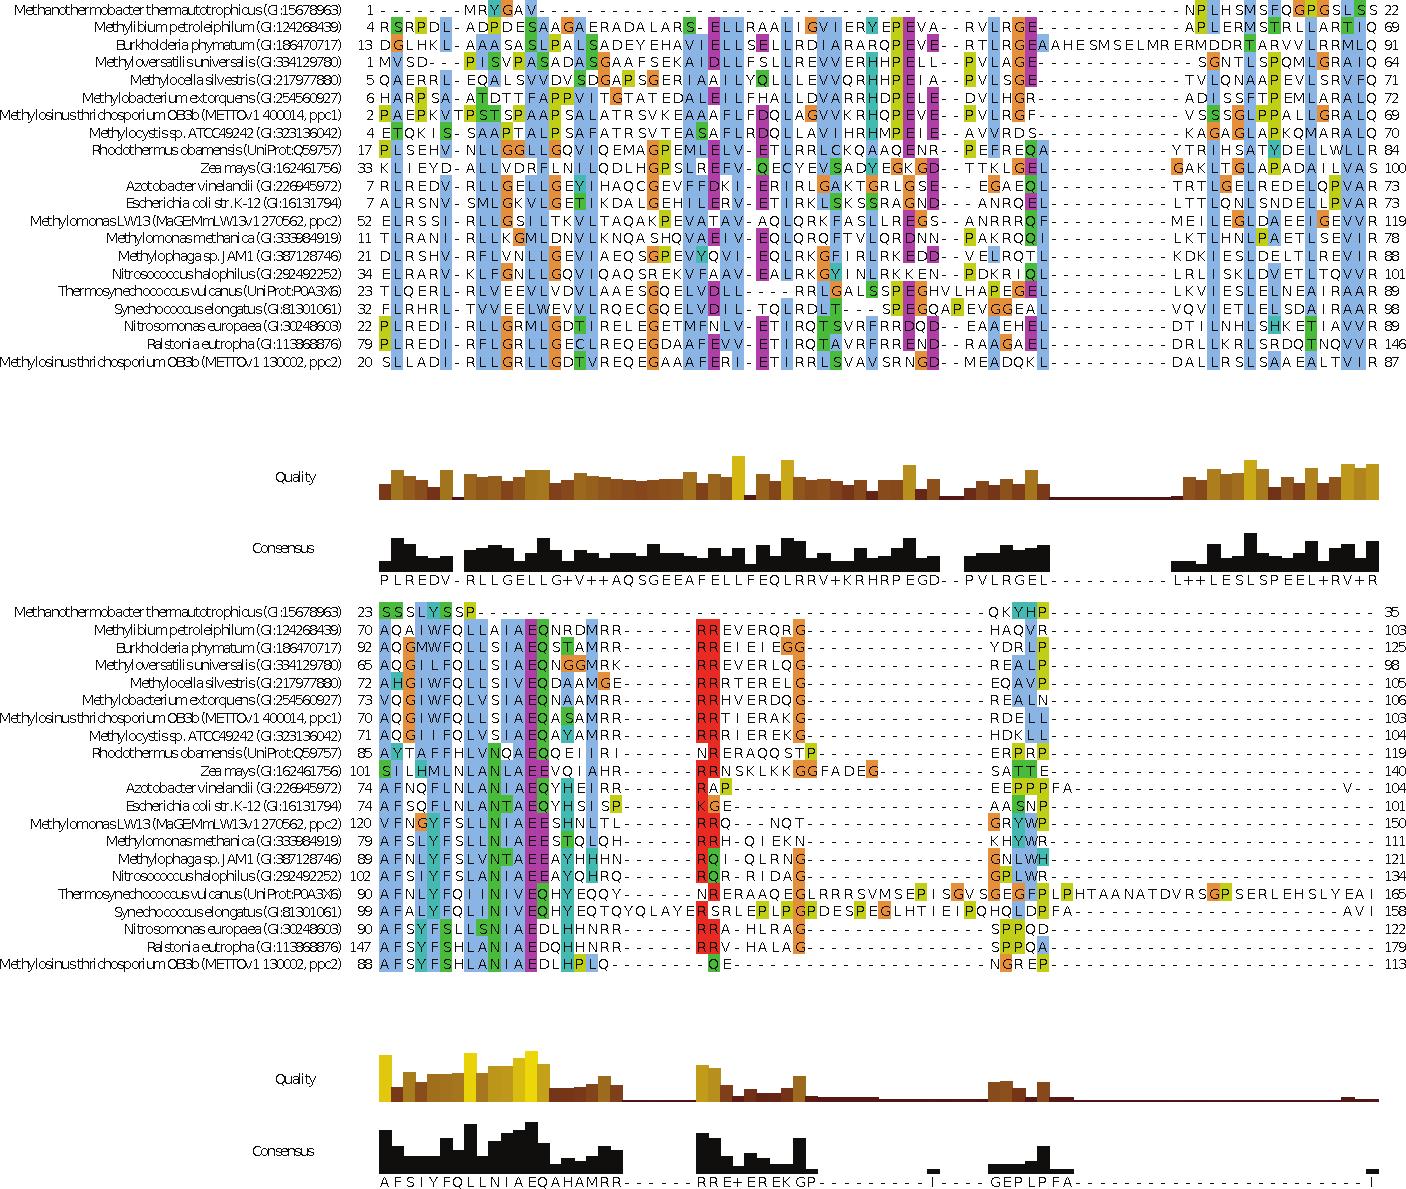
\includegraphics[width=1.0\textwidth]{./tex/chapter1/figures/supplemental/FigureS6a.pdf}
     \begin{singlespace}
     \caption[Structure alignment for phosphoenolpyruvate carboxylases (Ppc1 and Ppc2) from \textit{M. trichosporium OB3b} and Ppc-homologs]{
        Primary structure alignment for phosphoenolpyruvate carboxylases (Ppc1 and Ppc2) from \textit{M. trichosporium OB3b} and Ppc-homologs (continued on subsequent pages).
        }
     \label{fig:S6} % label before \end{singlespace} or references break.
     \end{singlespace}
\end{figure}

\begin{figure}[H]
\centering
     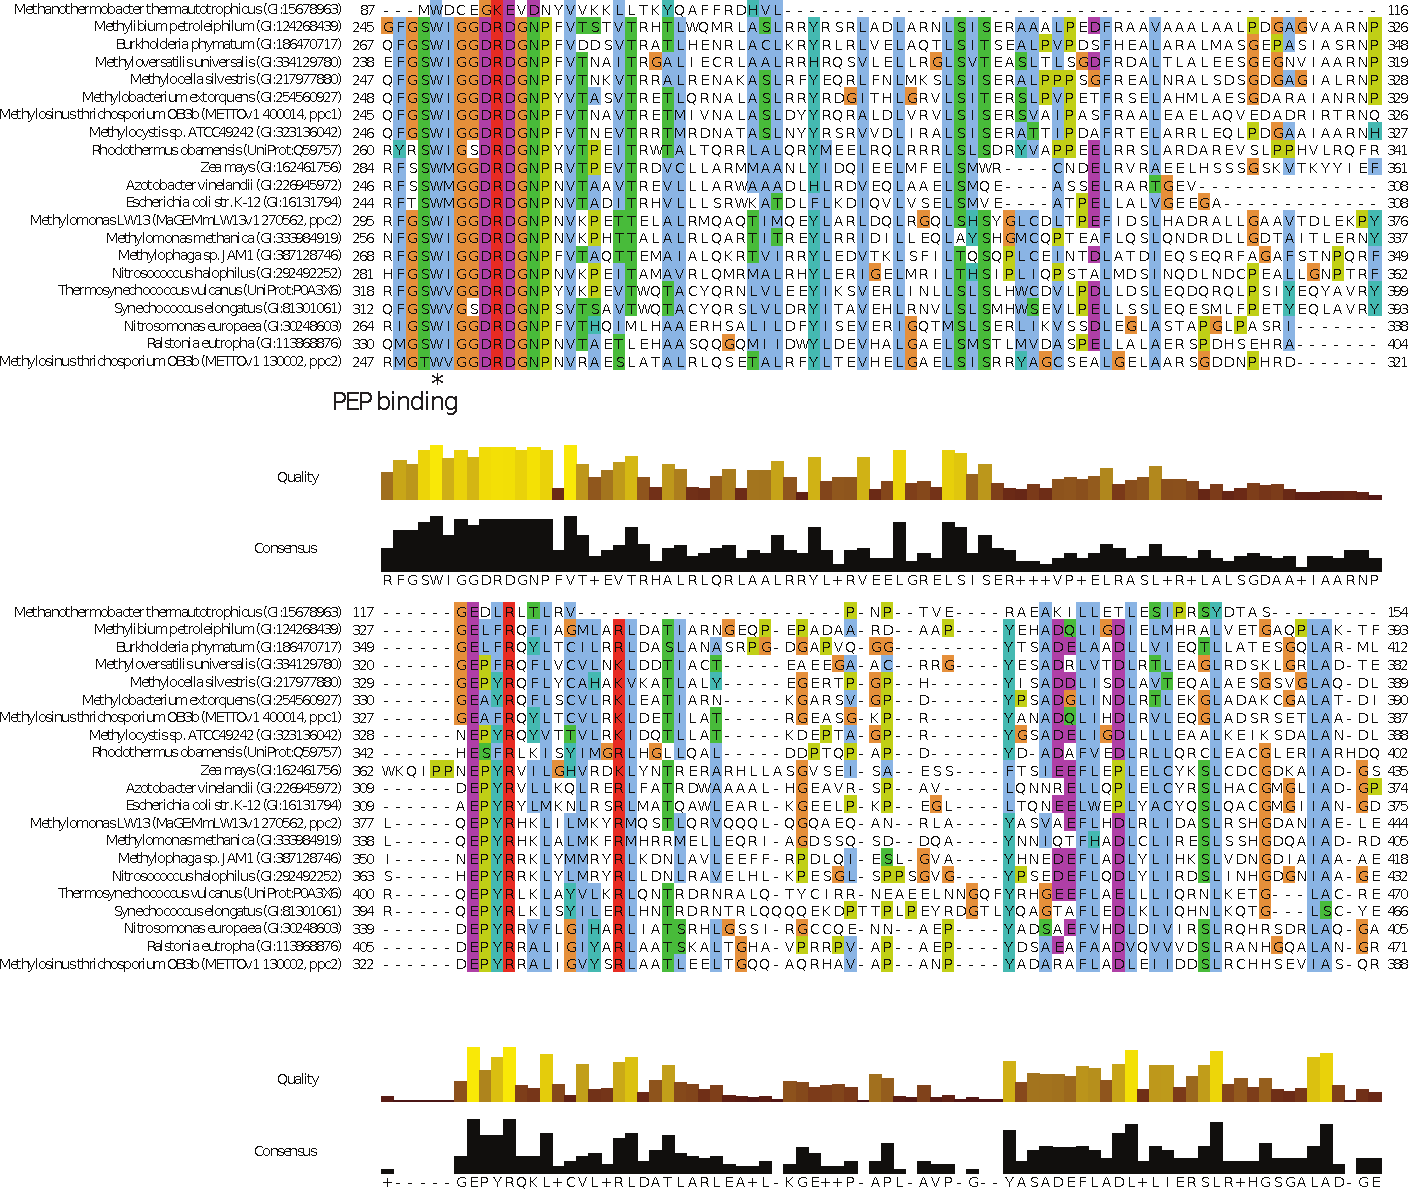
\includegraphics[width=1.0\textwidth]{./tex/chapter1/figures/supplemental/FigureS6c.pdf}
\end{figure}

\begin{figure}[H]
\centering
     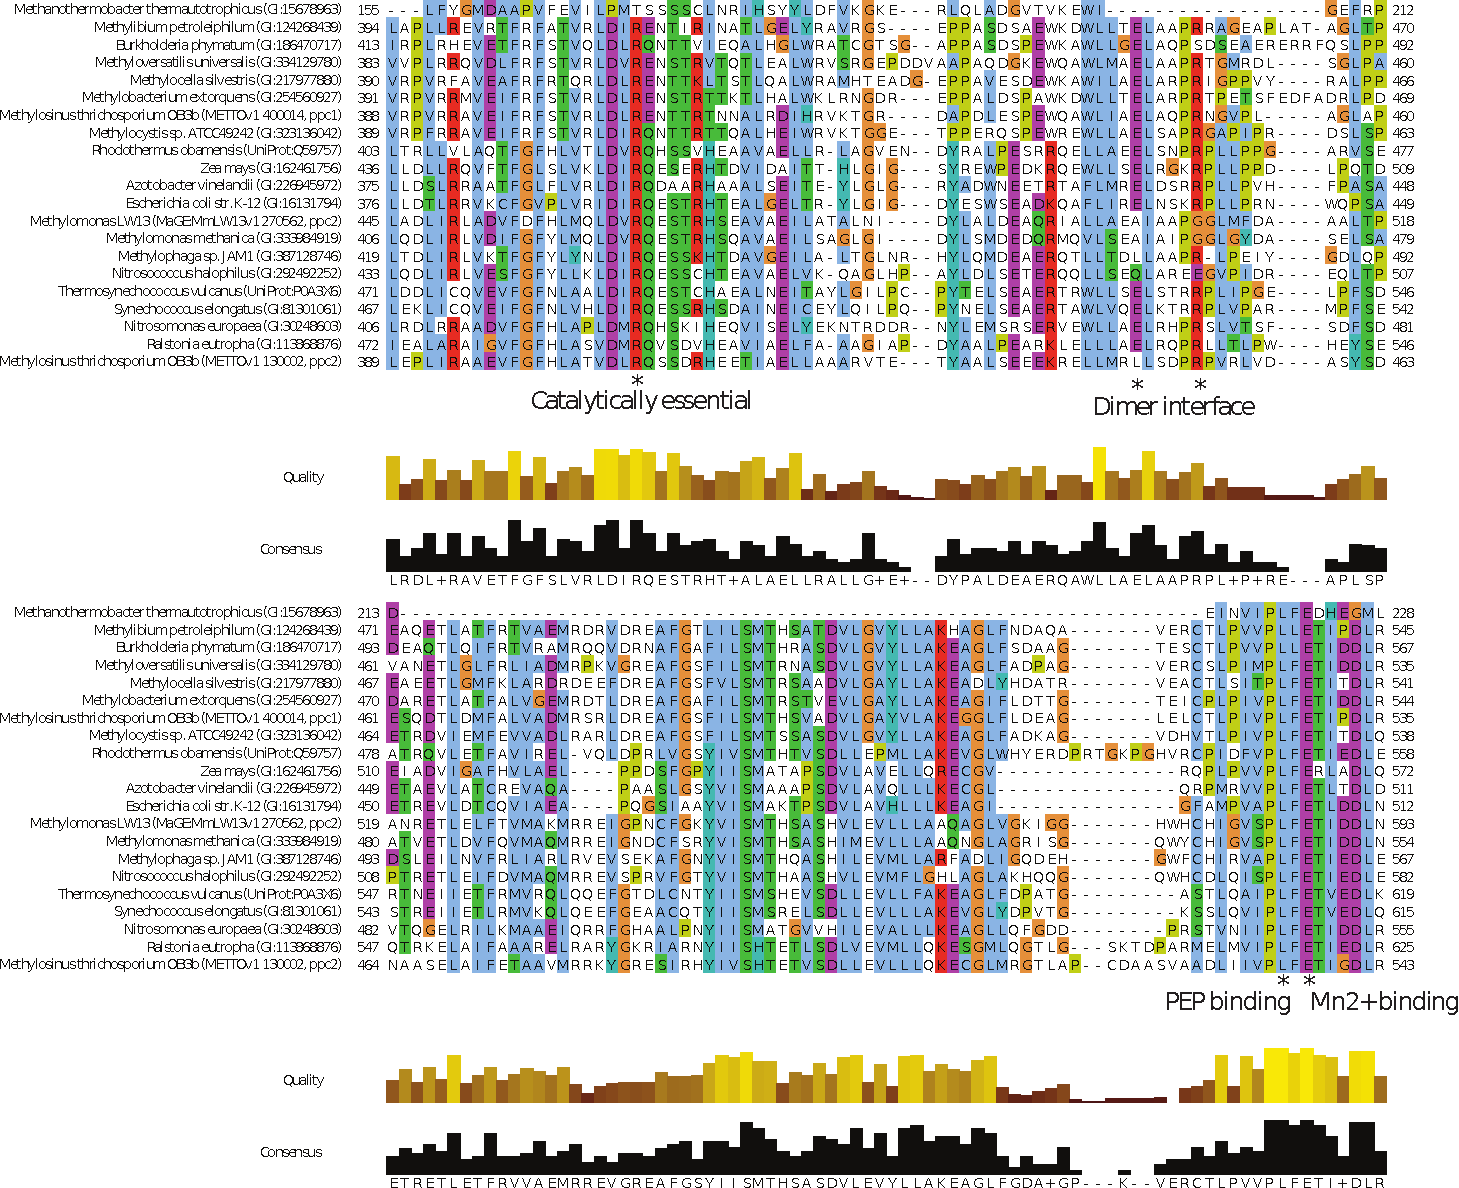
\includegraphics[width=1.0\textwidth]{./tex/chapter1/figures/supplemental/FigureS6d.pdf}
\end{figure}

\begin{figure}[H]
\centering
     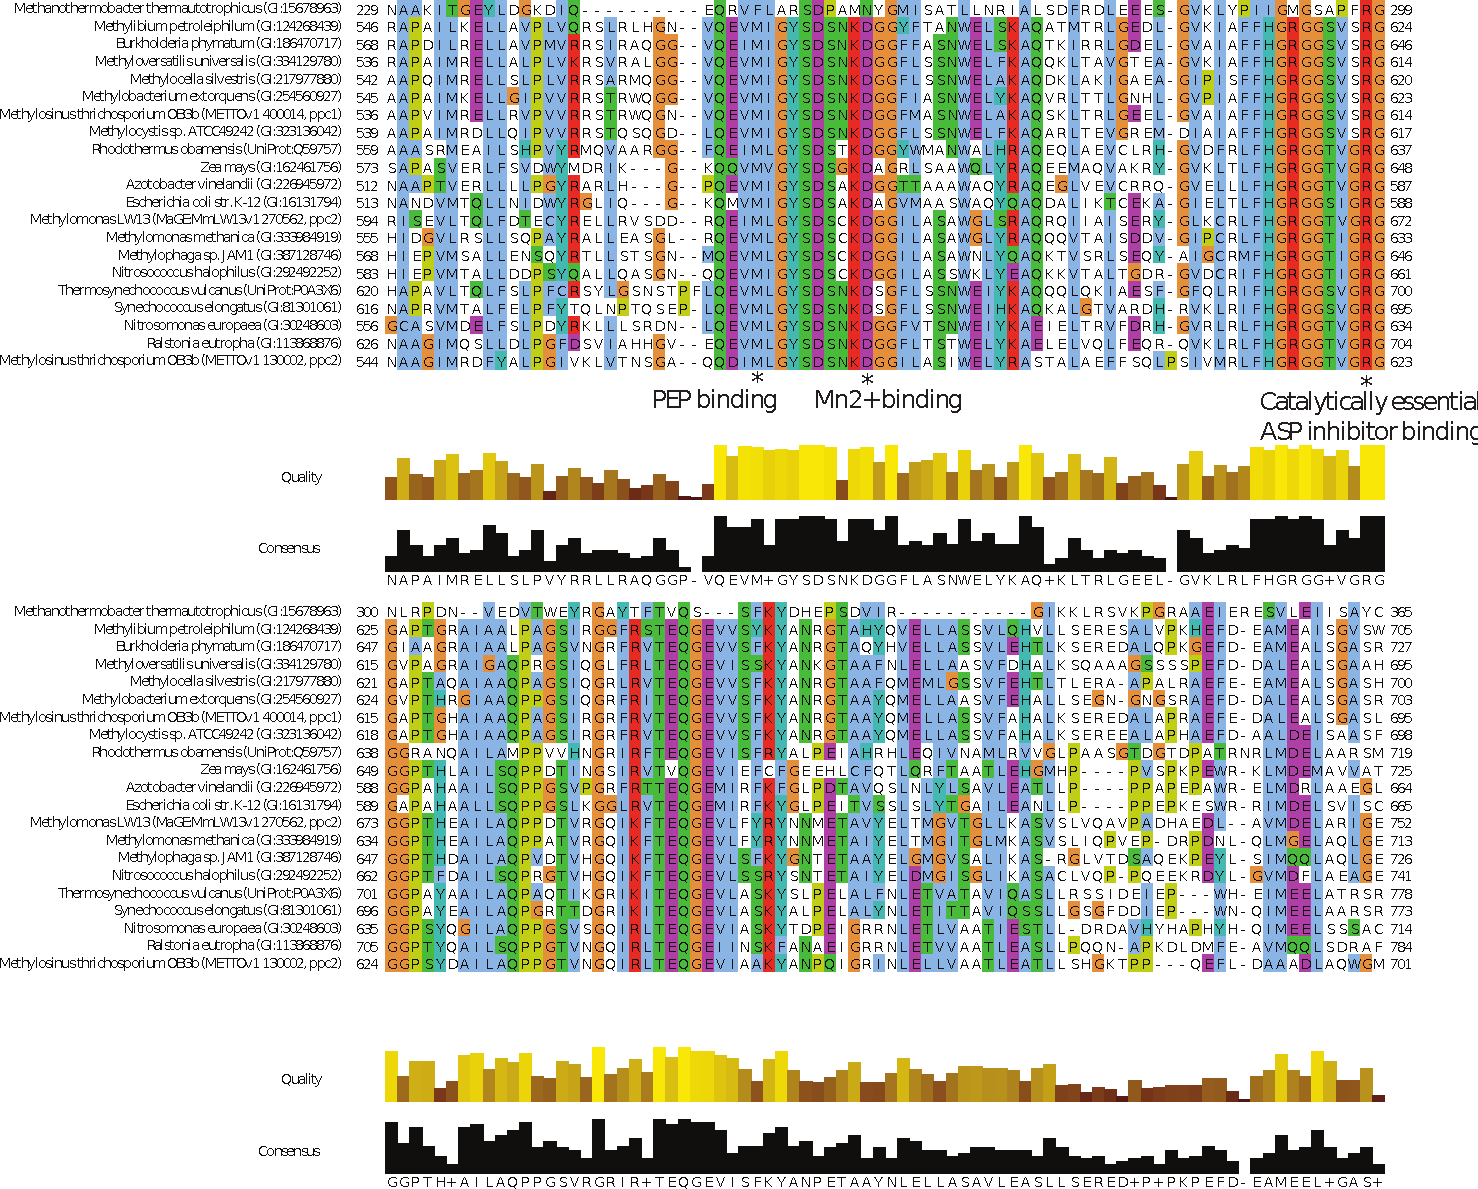
\includegraphics[width=1.0\textwidth]{./tex/chapter1/figures/supplemental/FigureS6e.pdf}
\end{figure}

\begin{figure}[H]
\centering
     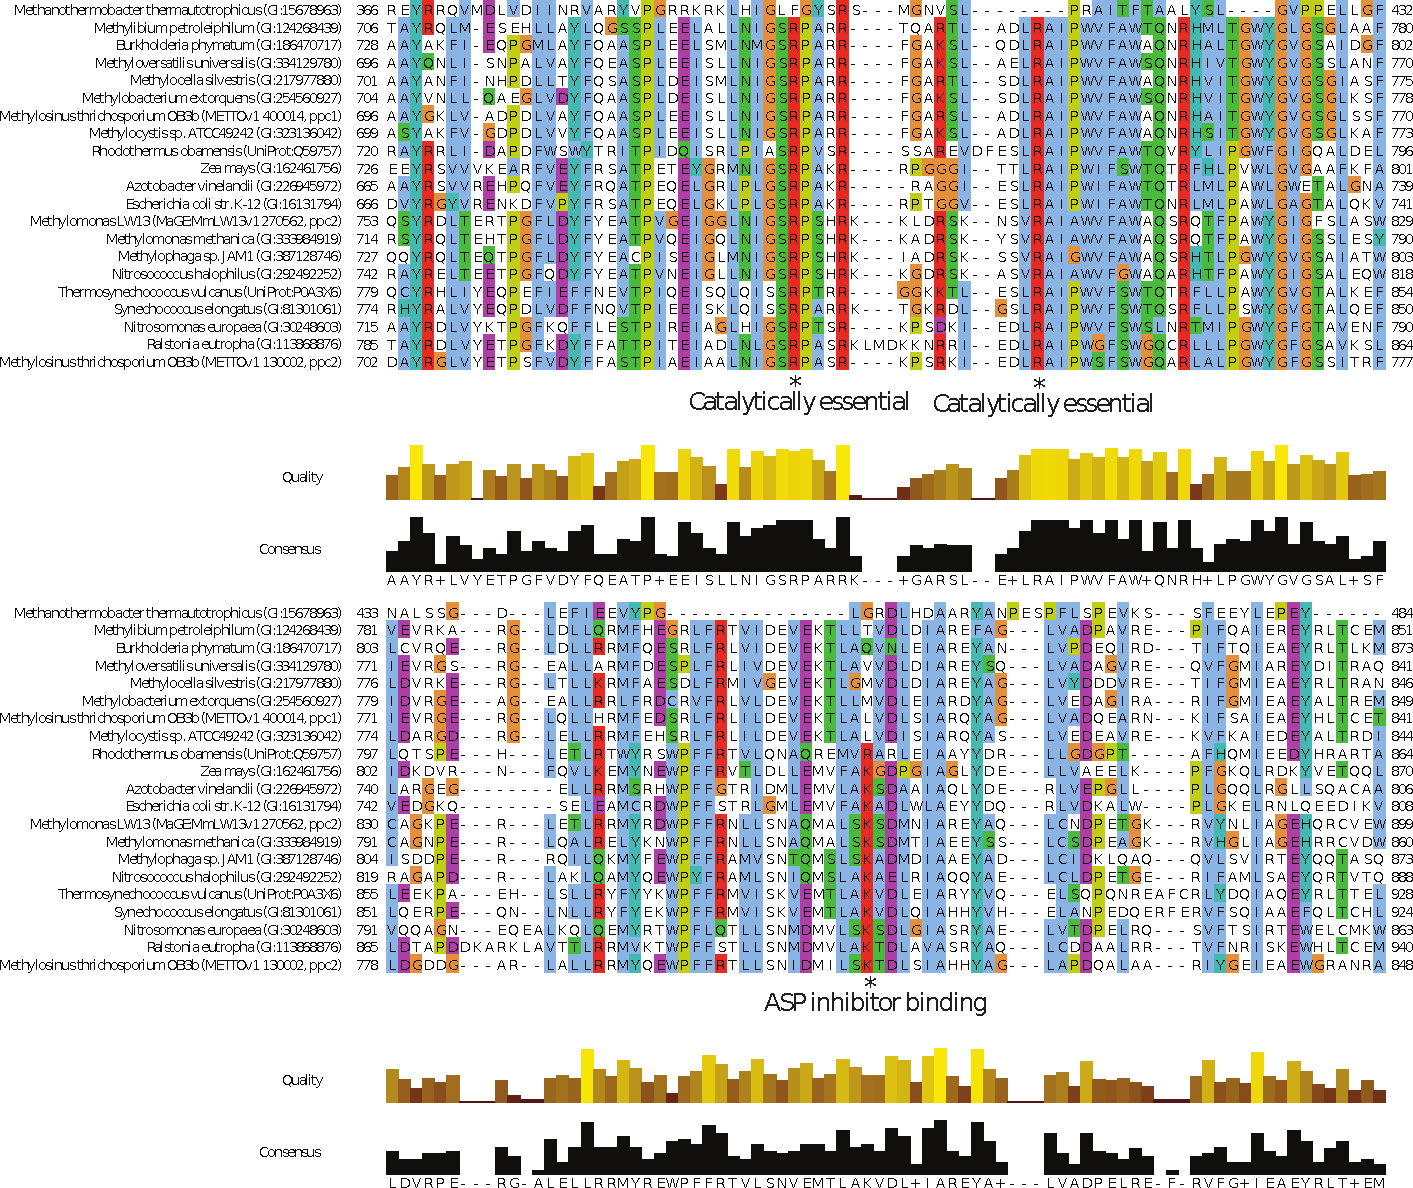
\includegraphics[width=1.0\textwidth]{./tex/chapter1/figures/supplemental/FigureS6f.pdf}
\end{figure}


\begin{figure}[H]
\centering
     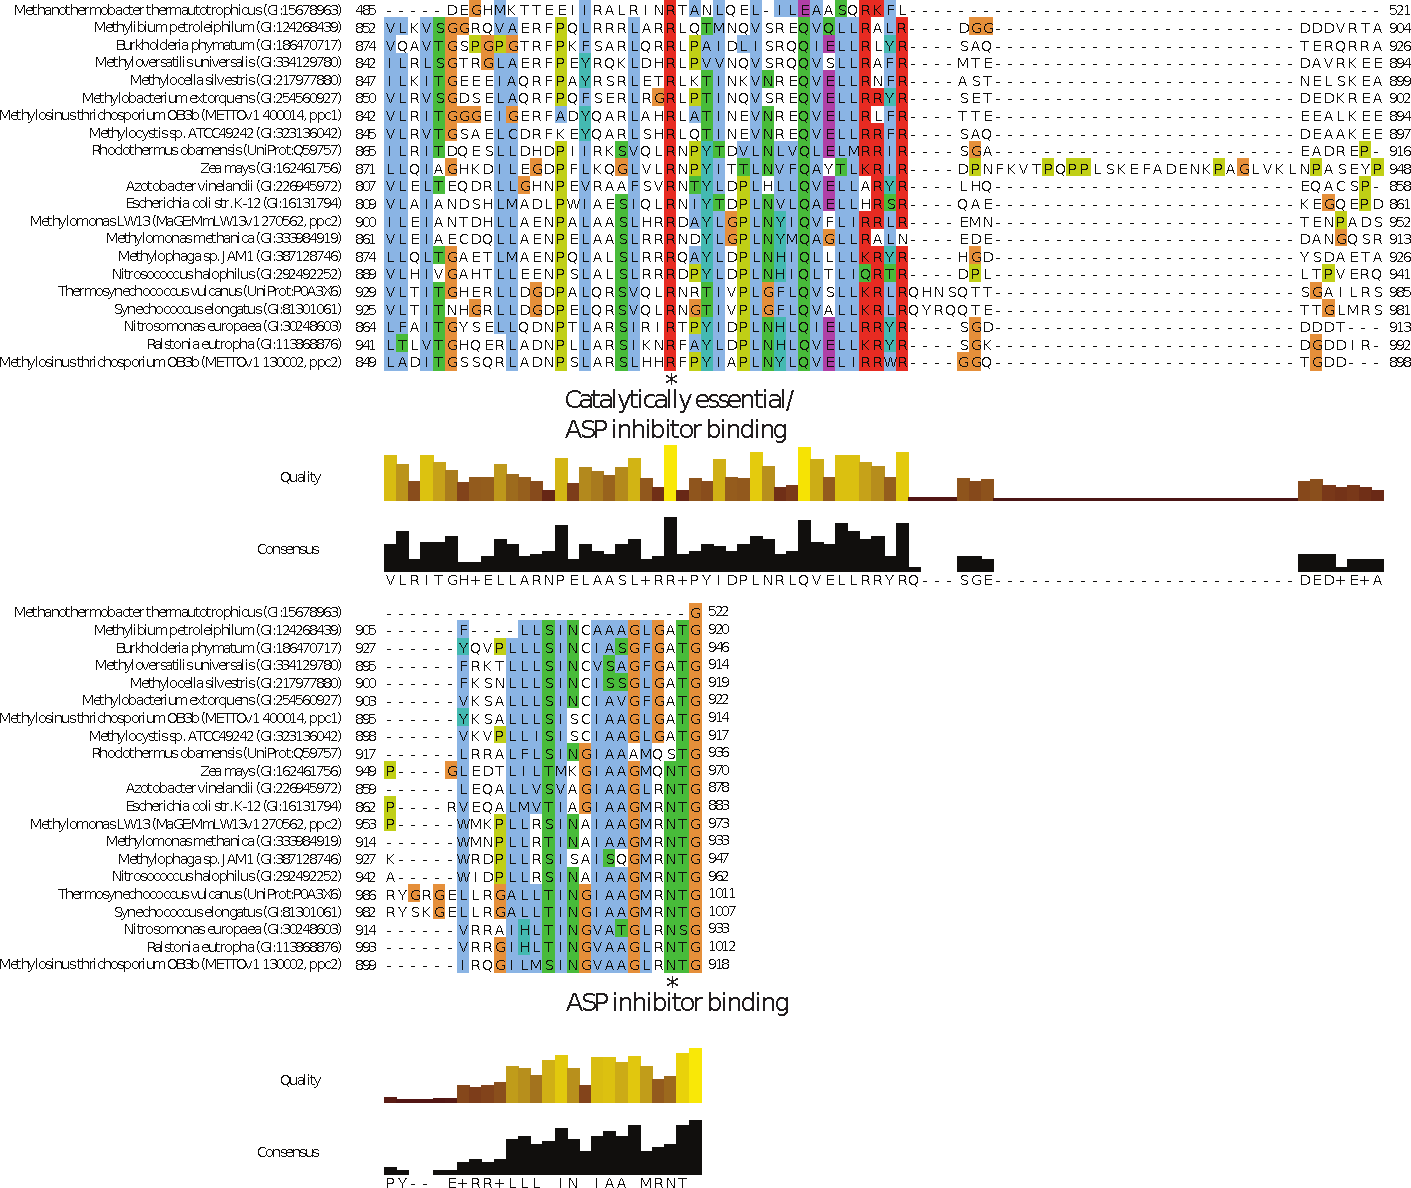
\includegraphics[width=1.0\textwidth]{./tex/chapter1/figures/supplemental/FigureS6g.pdf}
\end{figure}


%----- Supplementary Tables (as images)

\begin{table}[H]
\caption{Transcripts detected by \textit{de novo} assembly RNA-seq data.}
\label{table:ChA_S1}
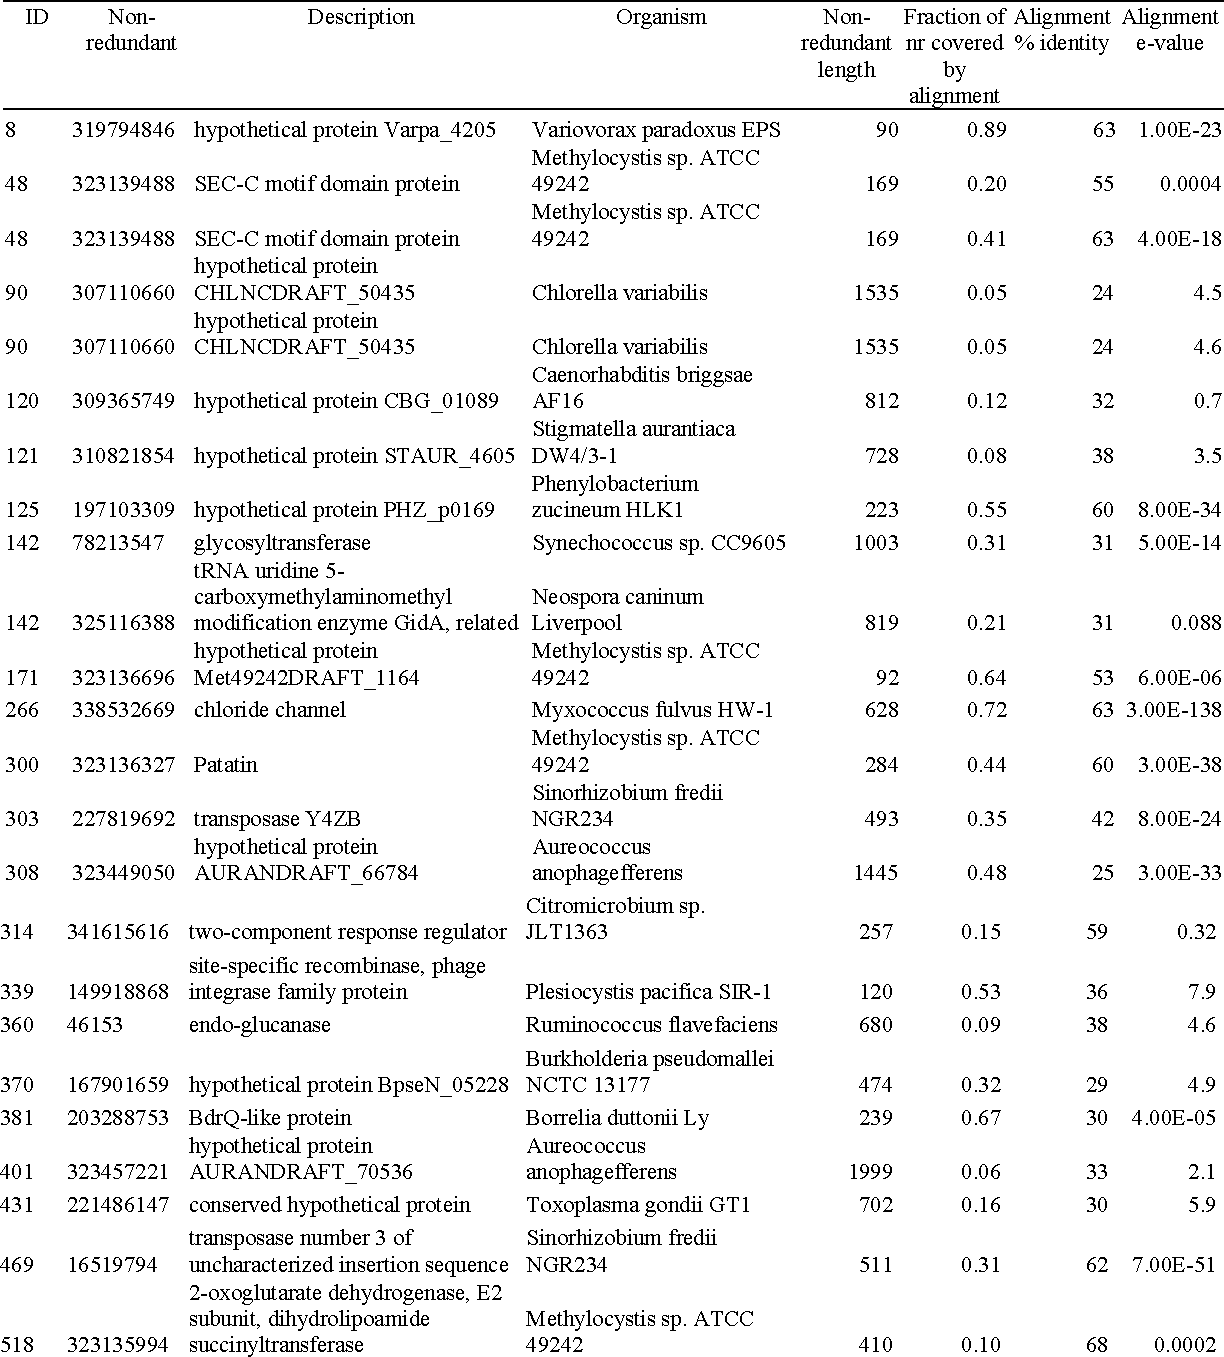
\includegraphics[width=1.0\textwidth]{./tex/chapter1/figures/supplemental/TableS1a.pdf}
\end{table}

%\begin{figure}[H]
%\centering
%    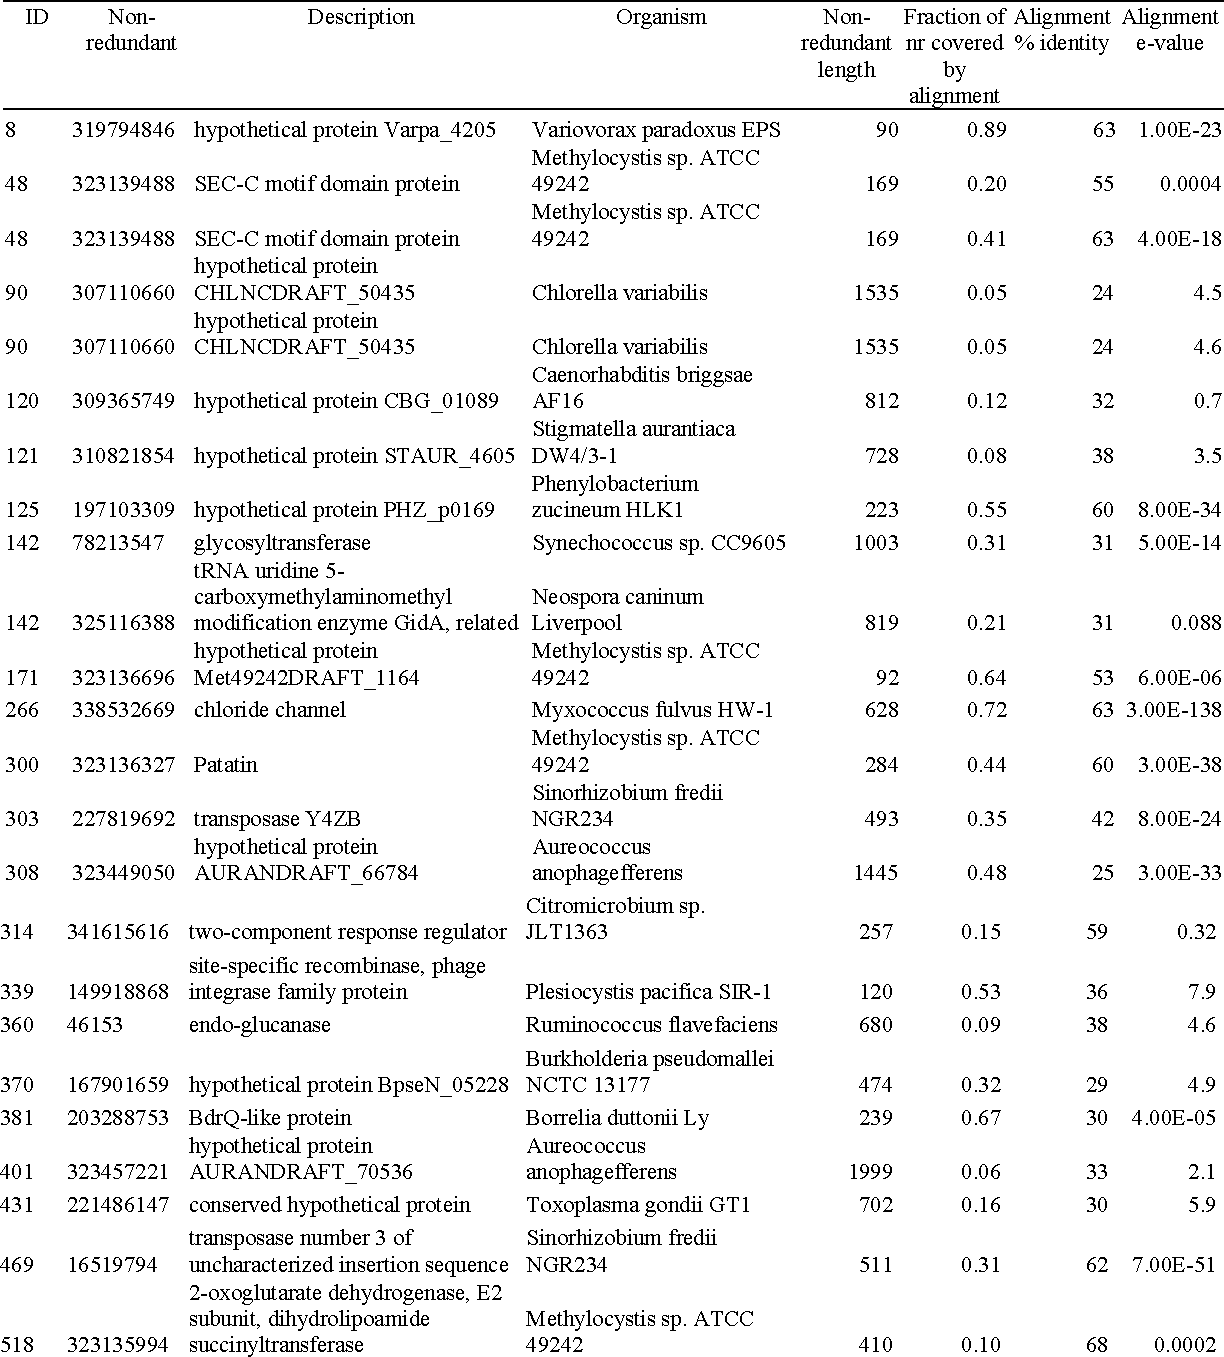
\includegraphics[width=1.0\textwidth]{./tex/chapter1/figures/supplemental/TableS1a.pdf}
%\end{figure}
\begin{figure}[H]
\centering
    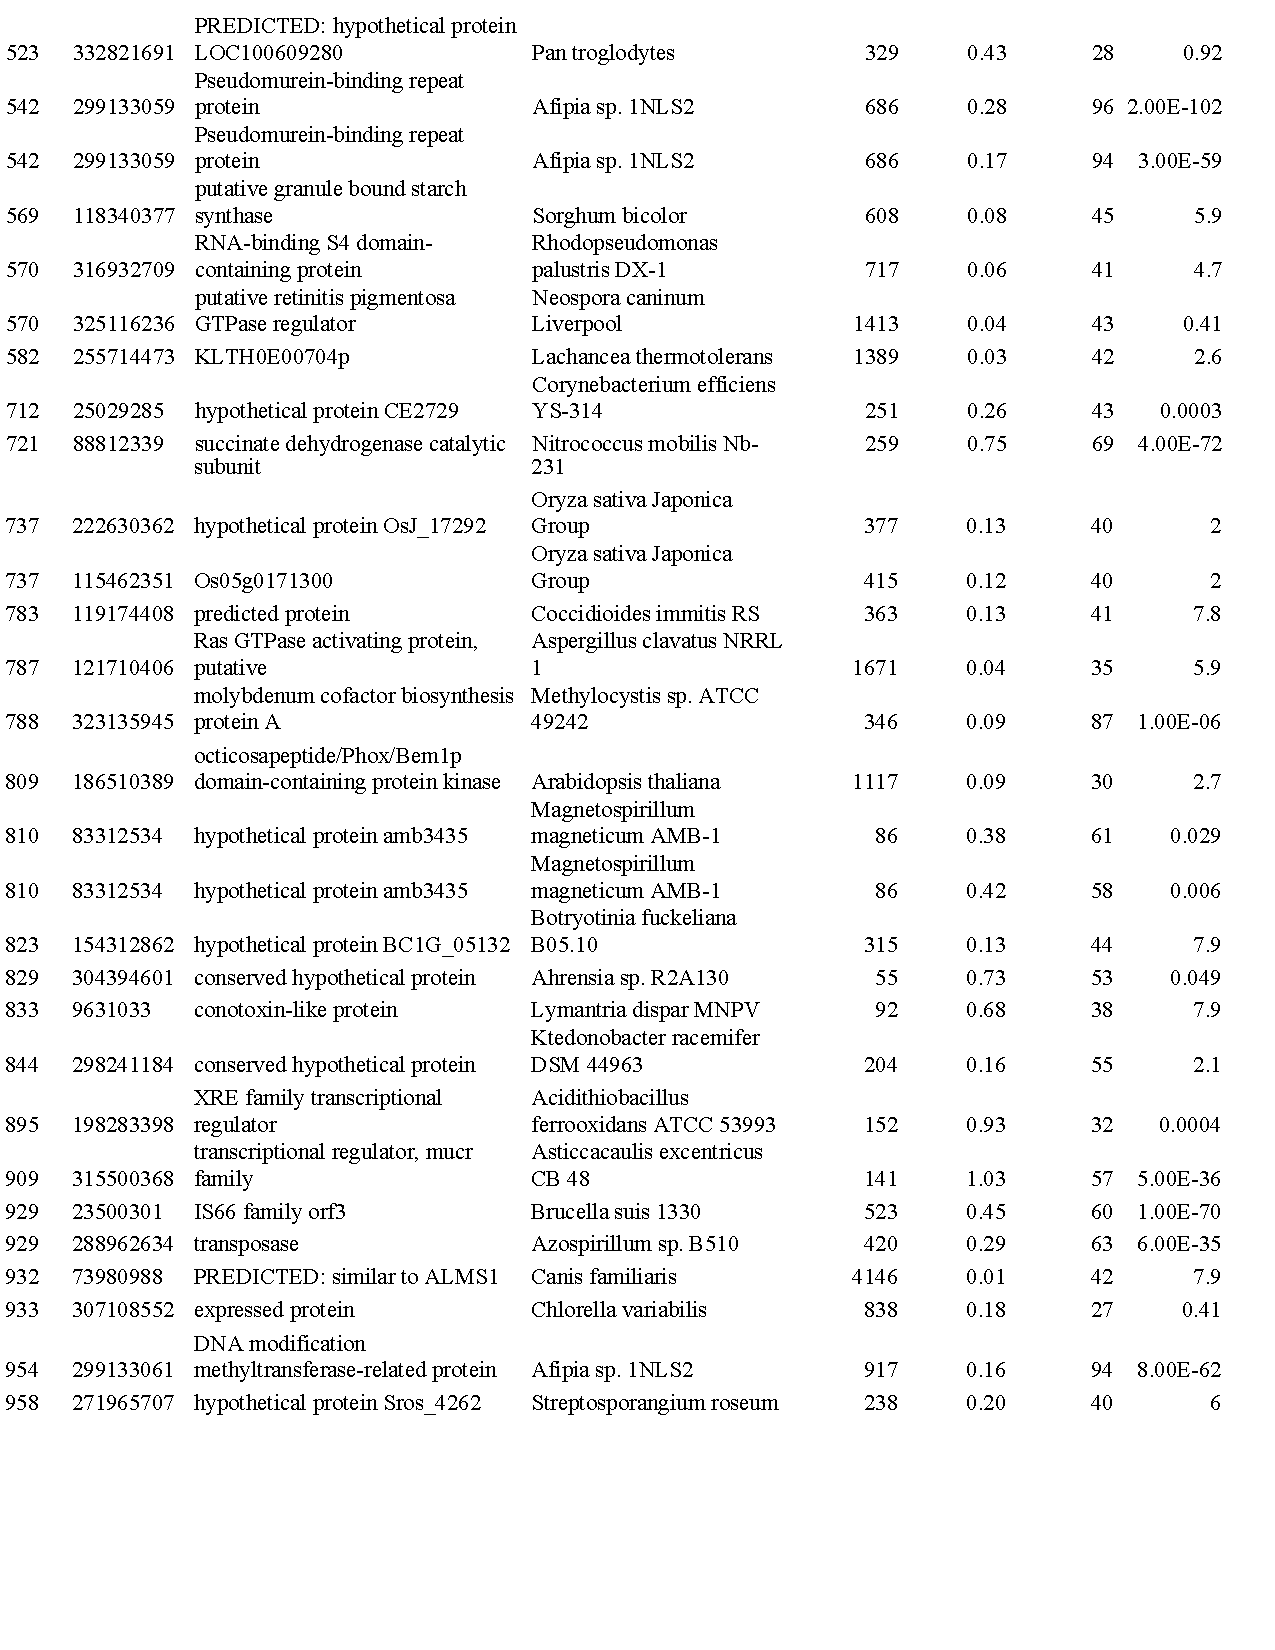
\includegraphics[width=1.0\textwidth]{./tex/chapter1/figures/supplemental/TableS1b.pdf}
\end{figure}
\begin{figure}[H]
\centering
    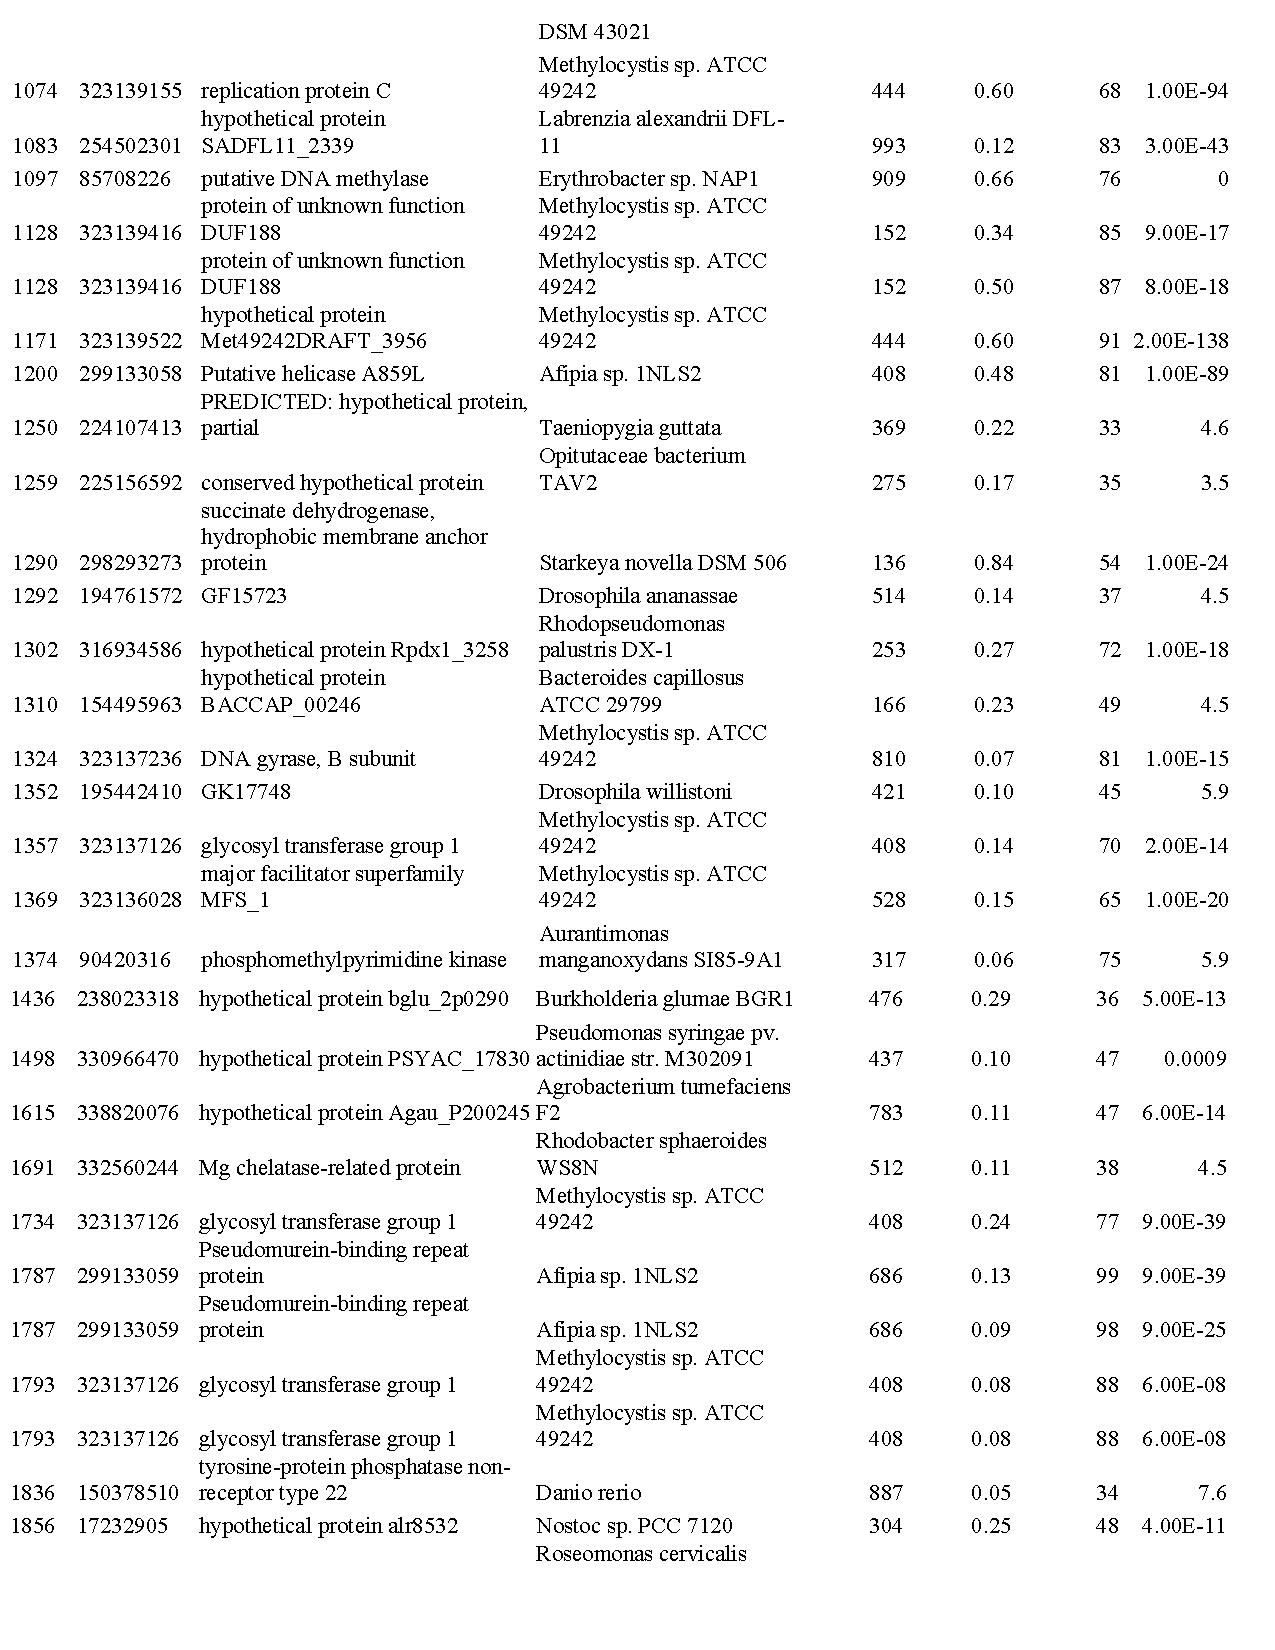
\includegraphics[width=1.0\textwidth]{./tex/chapter1/figures/supplemental/TableS1c.pdf}
\end{figure}
\begin{figure}[H]
\centering
    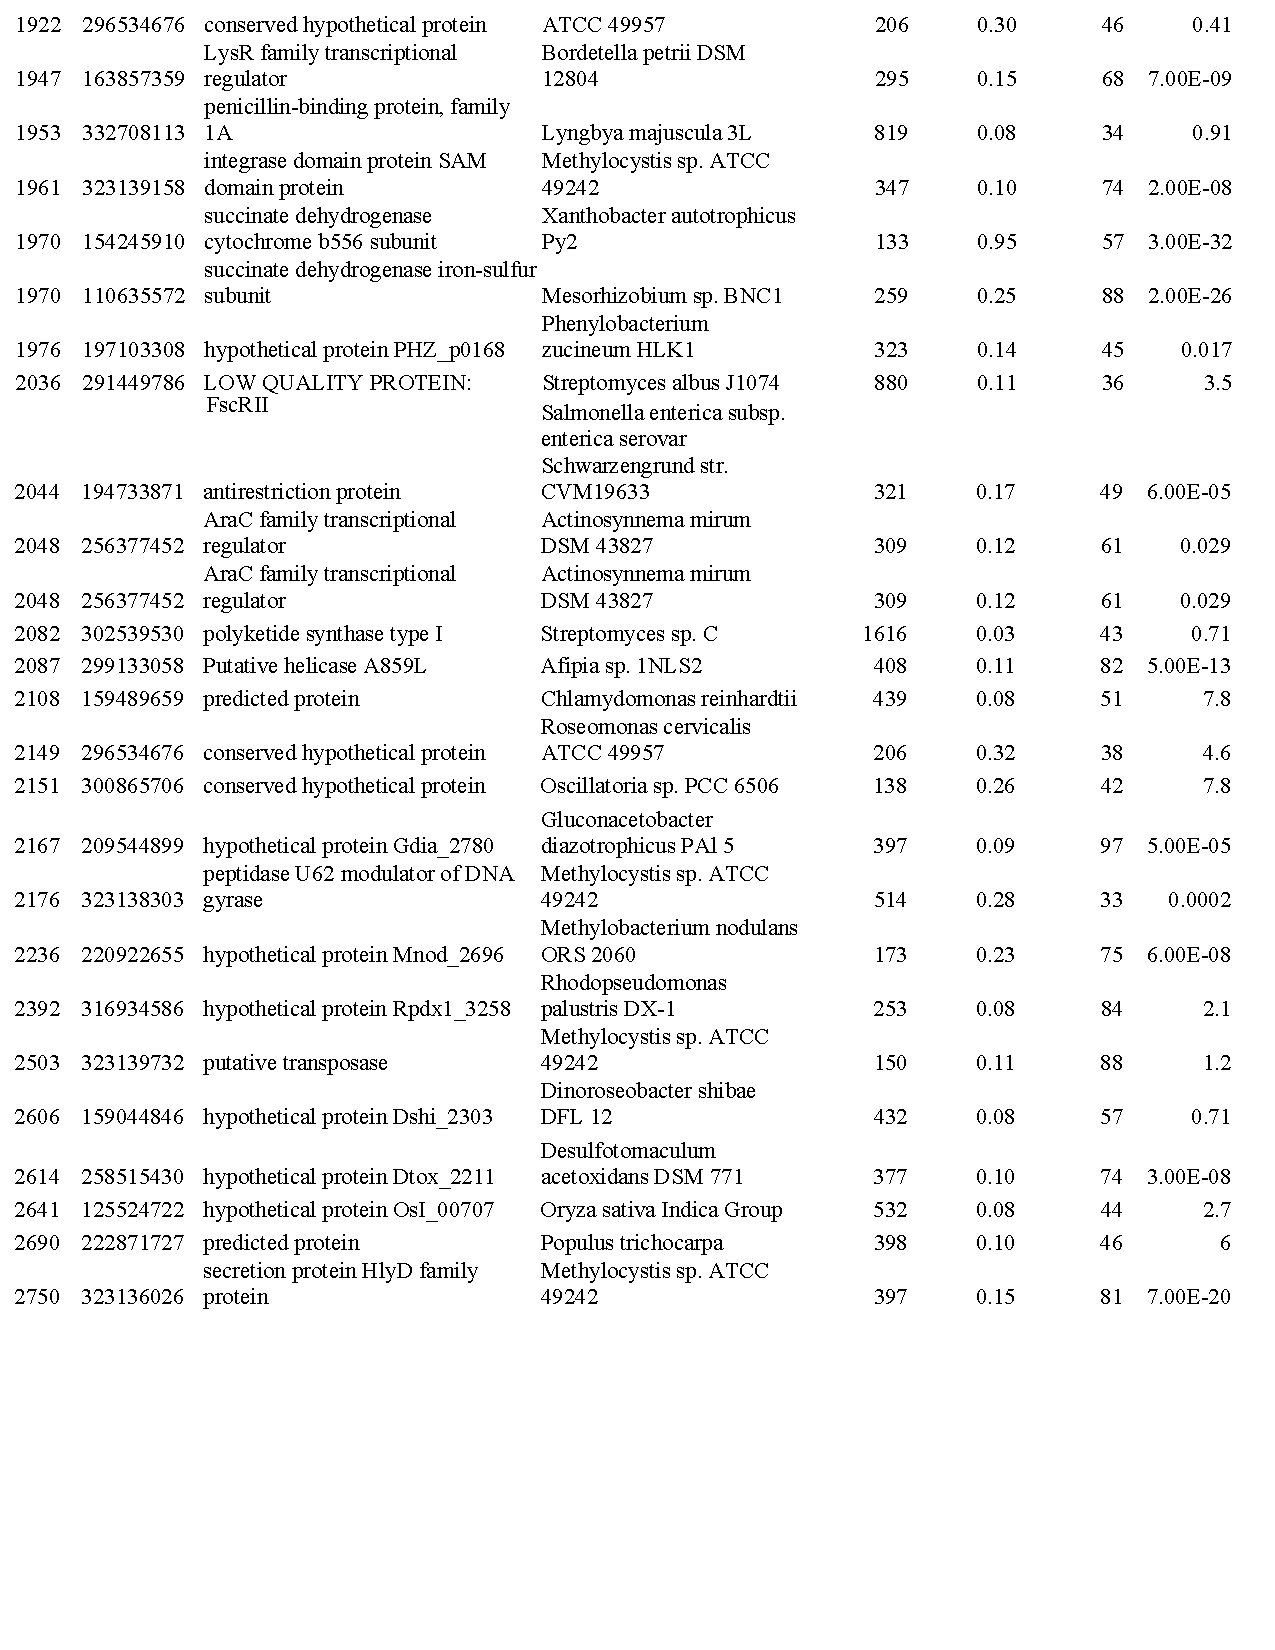
\includegraphics[width=1.0\textwidth]{./tex/chapter1/figures/supplemental/TableS1d.pdf}
\end{figure}
\begin{figure}[H]
\centering
    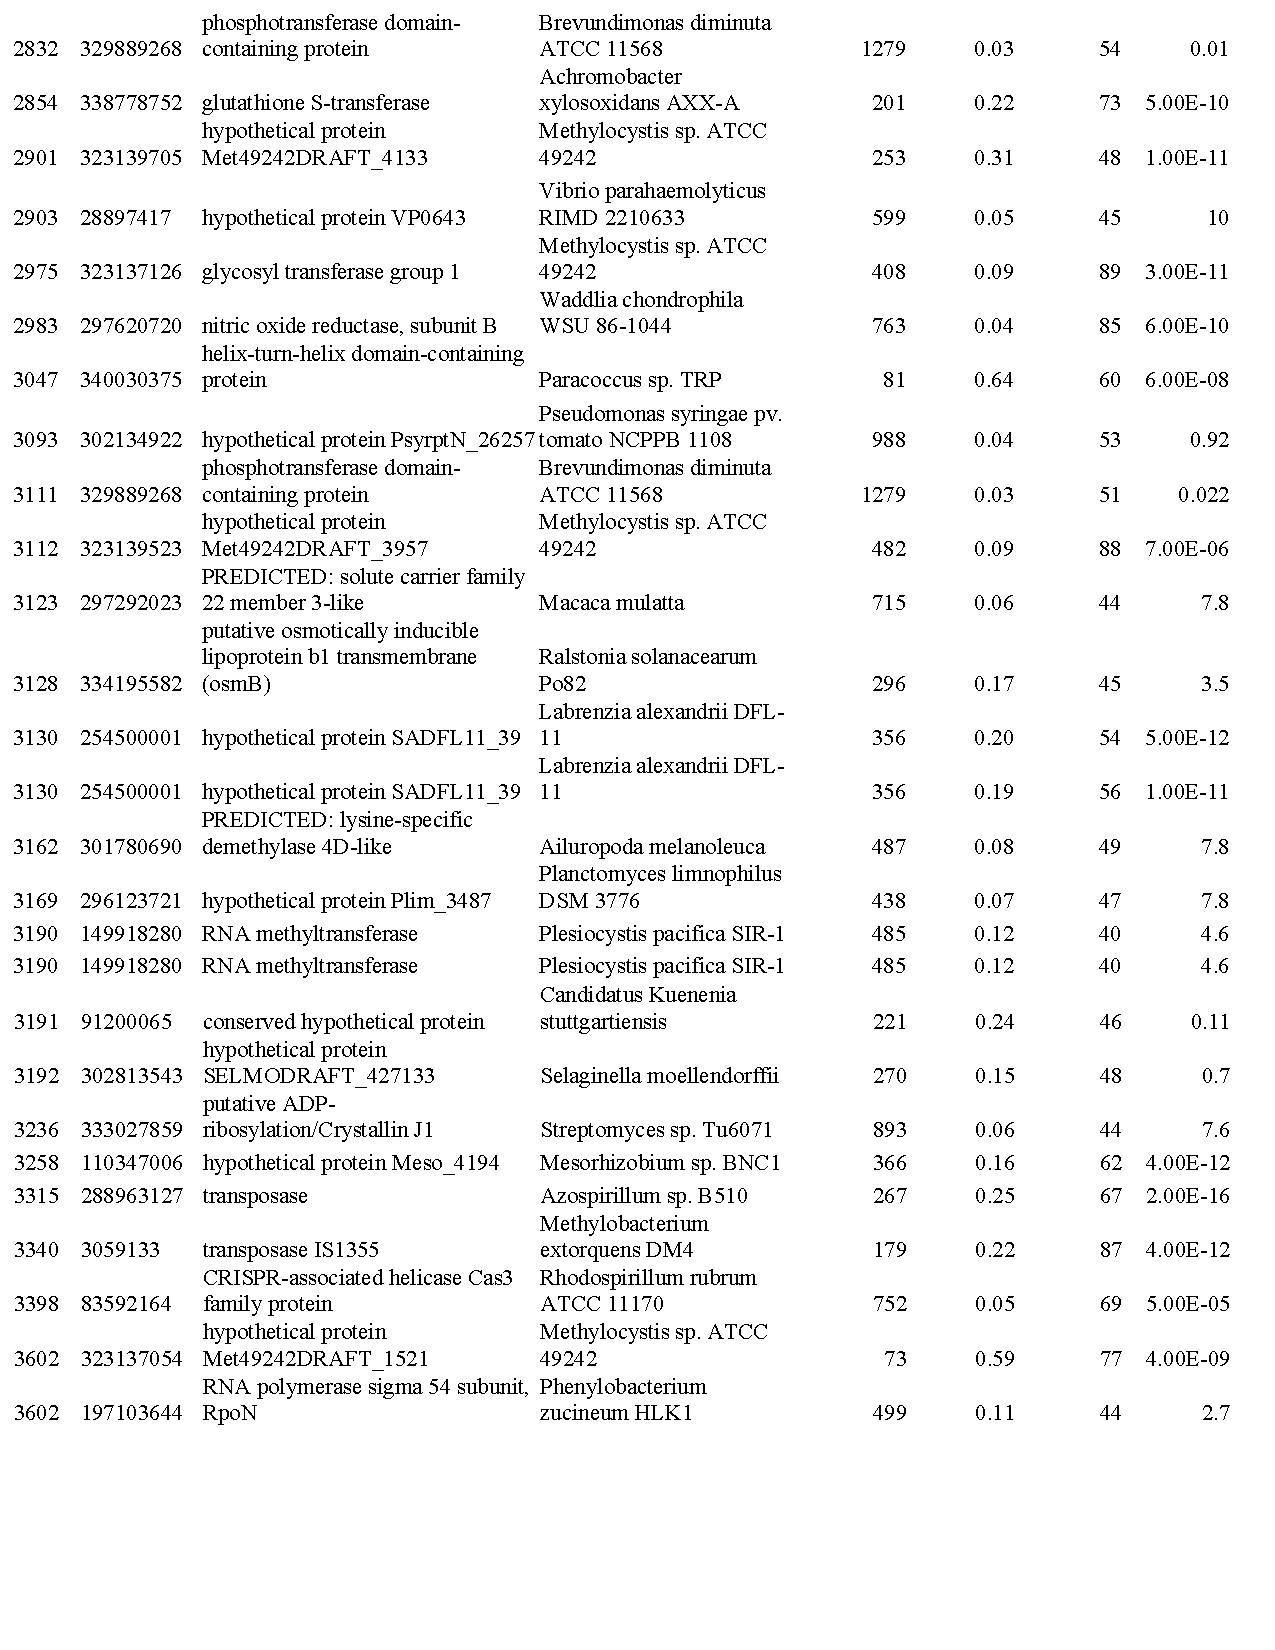
\includegraphics[width=1.0\textwidth]{./tex/chapter1/figures/supplemental/TableS1e.pdf}
\end{figure}
\begin{figure}[H]
\centering
    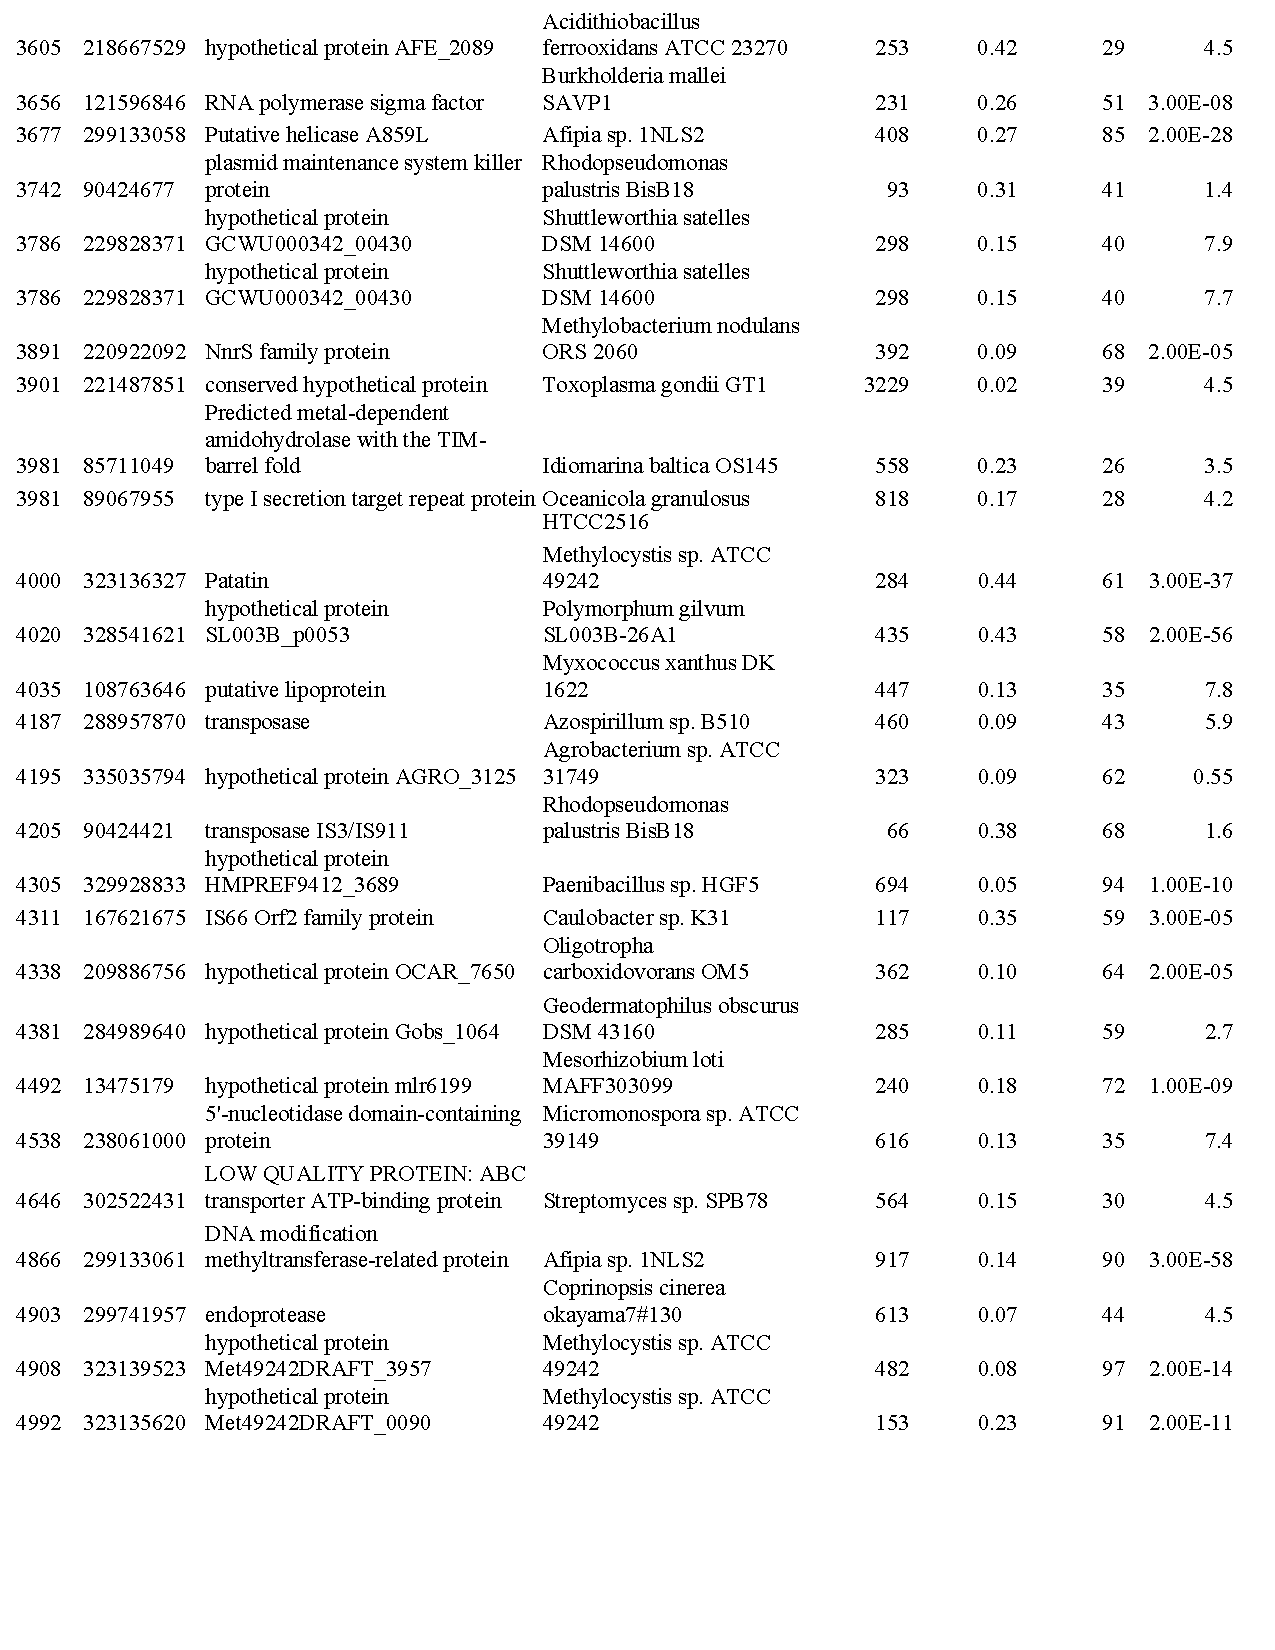
\includegraphics[width=1.0\textwidth]{./tex/chapter1/figures/supplemental/TableS1f.pdf}
\end{figure}
\begin{figure}[H]
\centering
    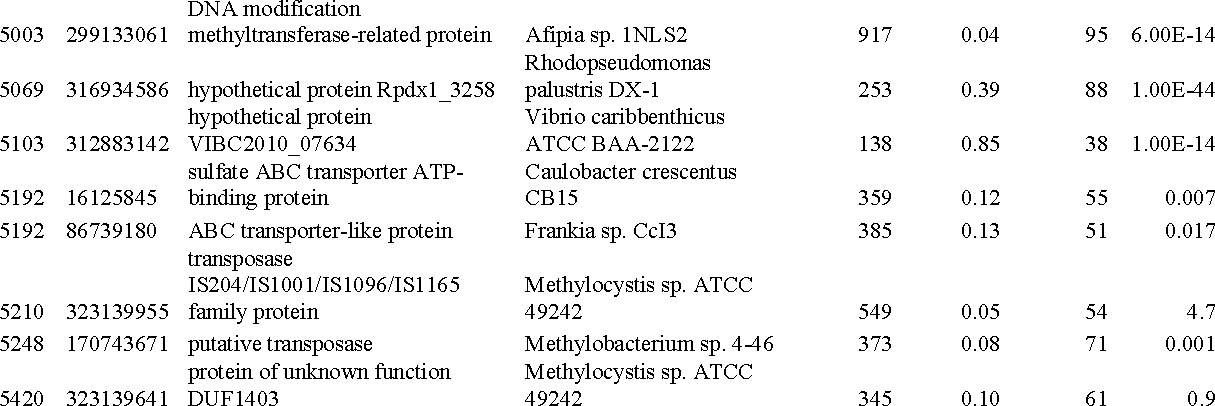
\includegraphics[width=1.0\textwidth]{./tex/chapter1/figures/supplemental/TableS1g.pdf}
\end{figure}


\begin{table}[H]
\begin{singlespace}
\caption[Methane-grown \textit{M. trichosporium OB3b} gene expression table (RPKM)]{
	Gene expression profile in methane-grown cells of \textit{M. trichosporium OB3b}.
	Values represent reads per kilobase of coding sequence per million (reads) mapped (RPKM).
	For the full 4,812-row data set, see attached file.}
\label{table:ChA_S2}
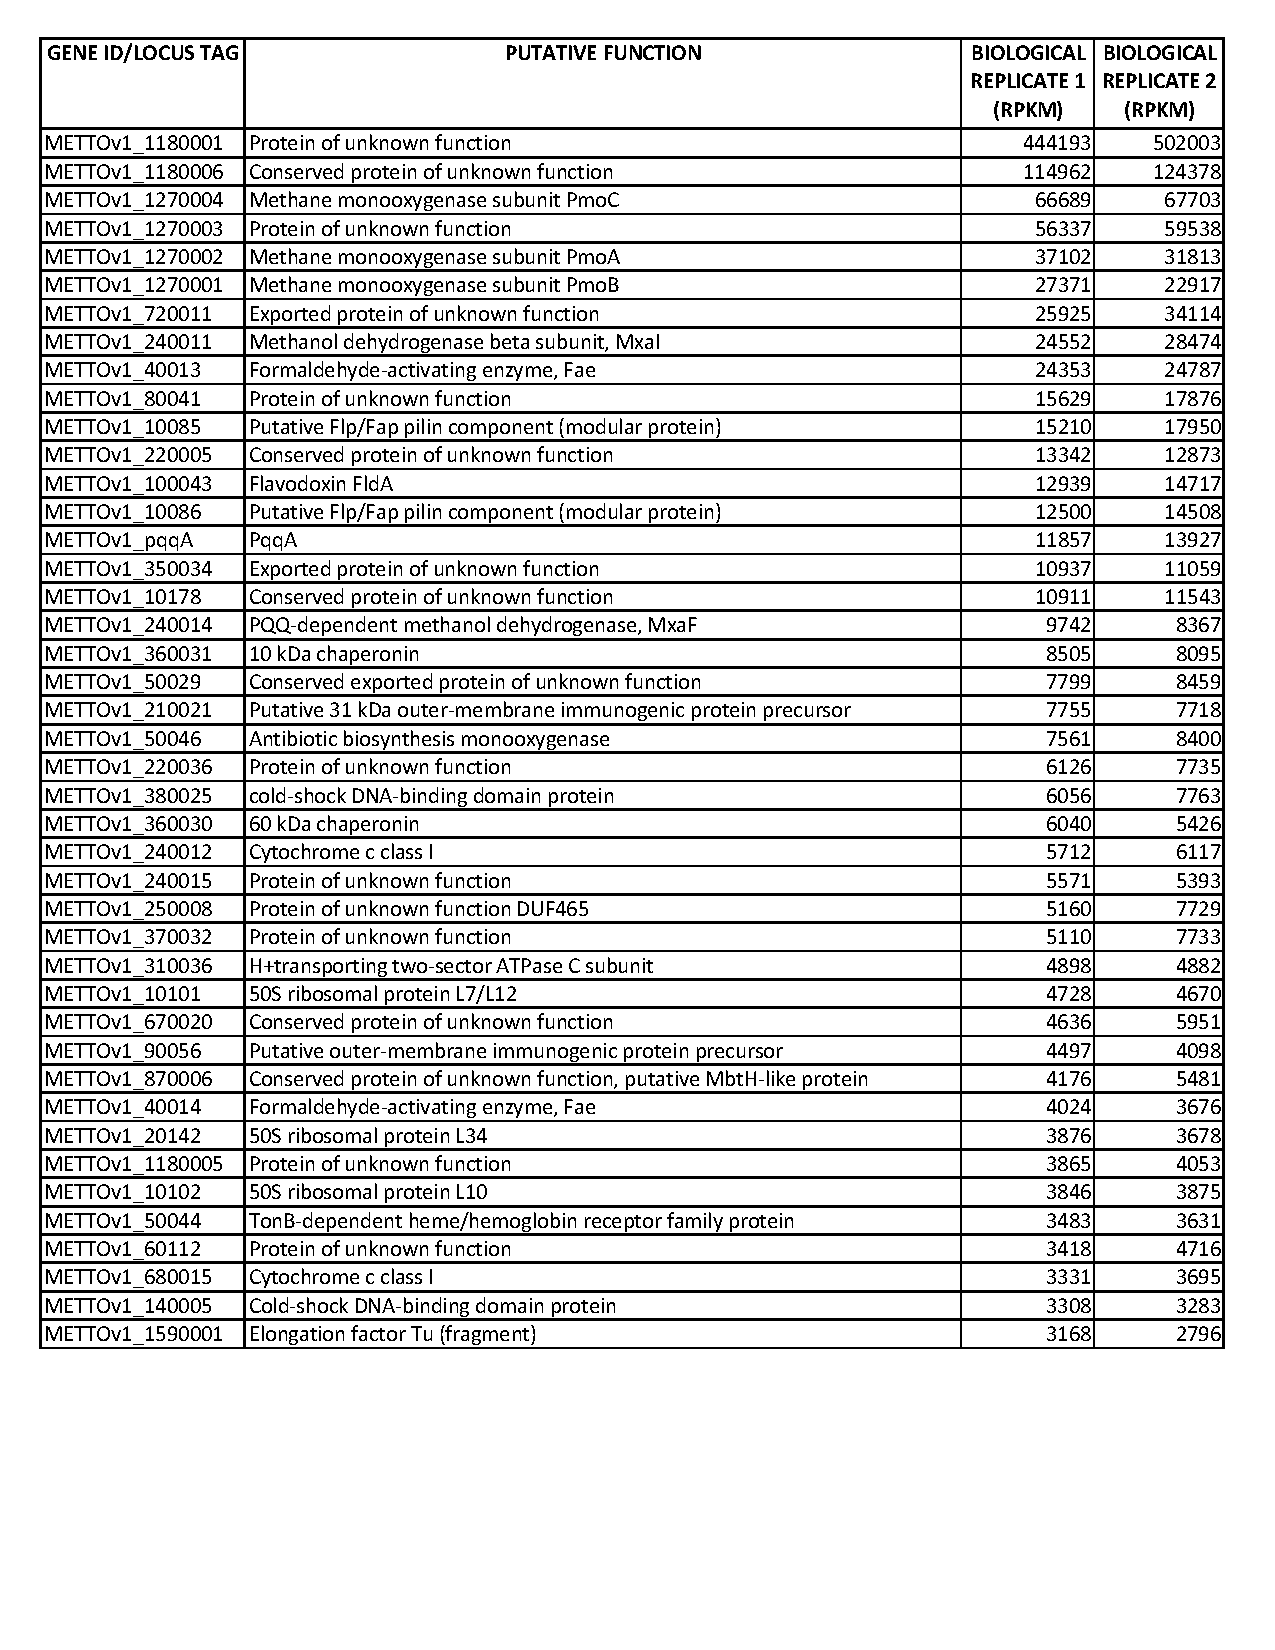
\includegraphics[width=1.0\textwidth]{./tex/chapter1/figures/supplemental/TableS2a.pdf}
\end{singlespace}
\end{table}
%---
\begin{figure}[H]
\centering
    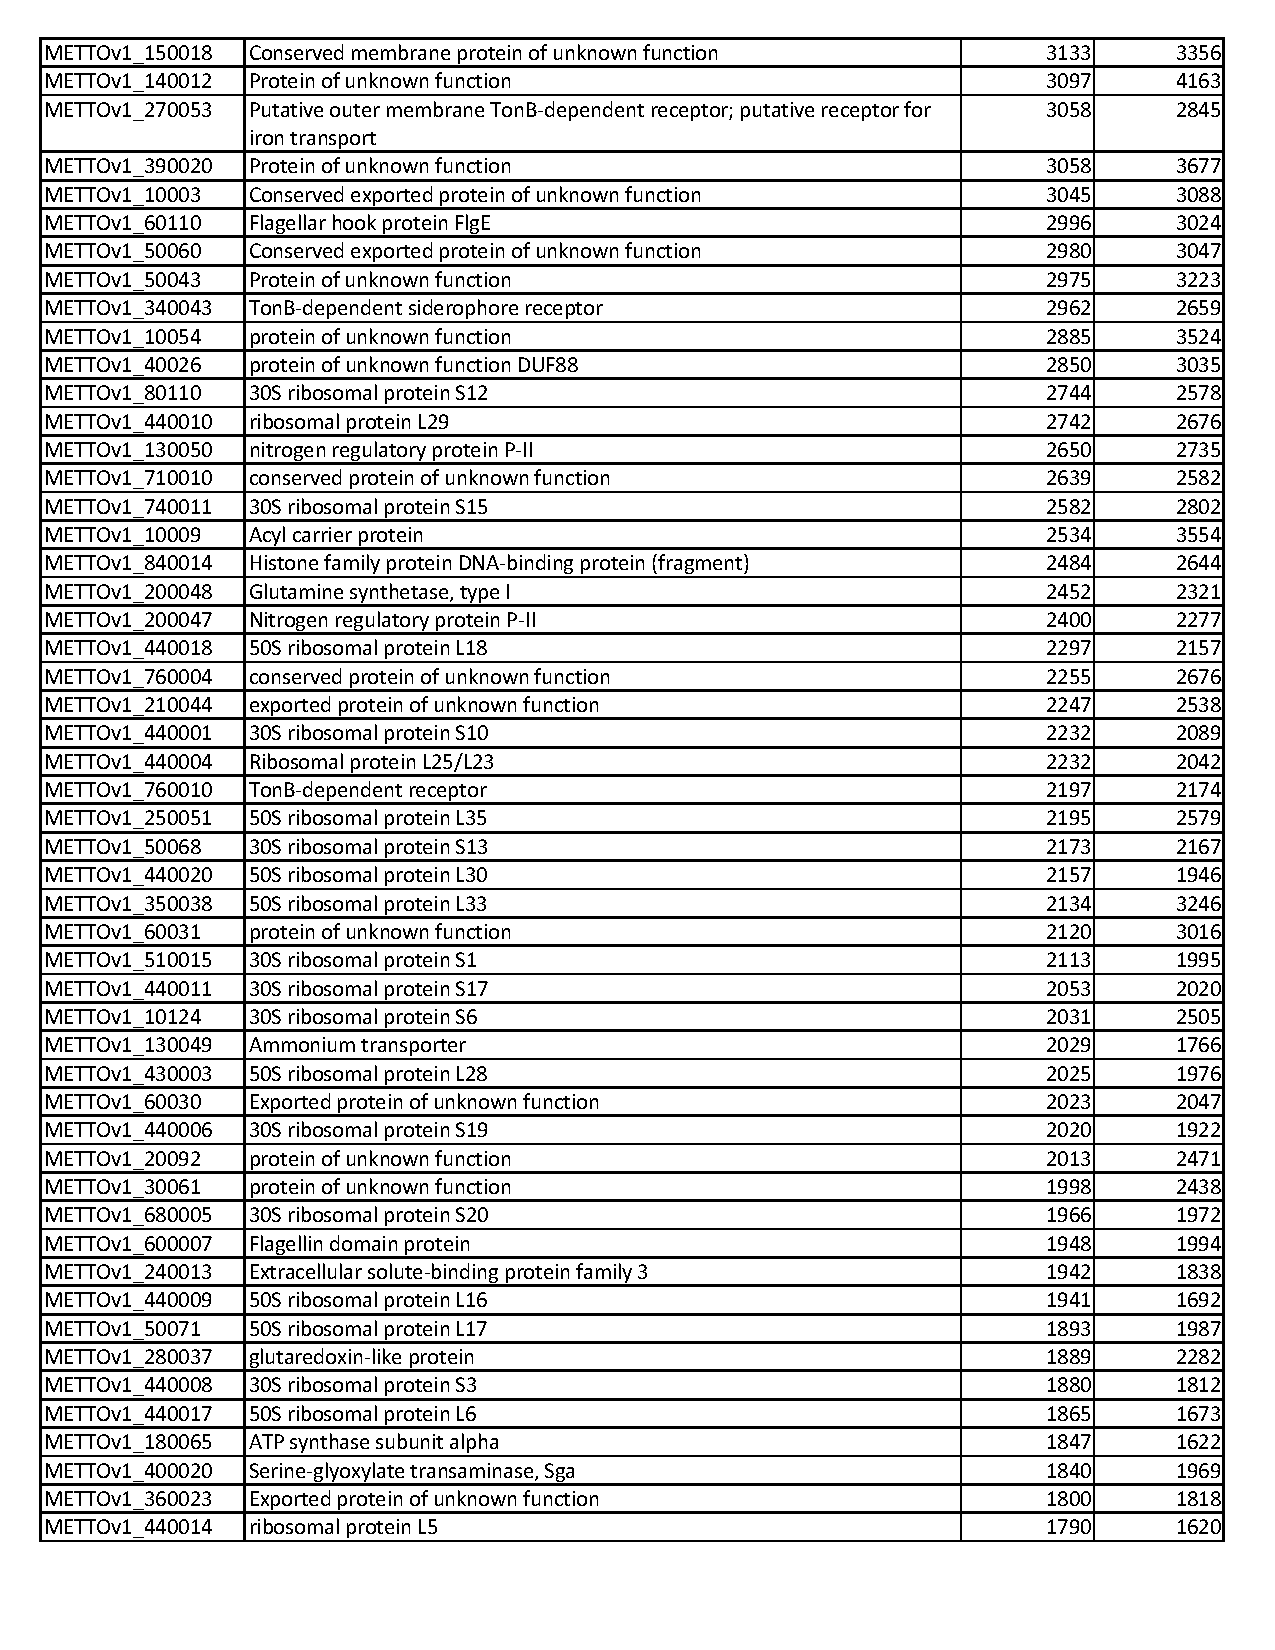
\includegraphics[width=1.0\textwidth]{./tex/chapter1/figures/supplemental/TableS2b.pdf}
\end{figure}
\begin{figure}[H]
\centering
    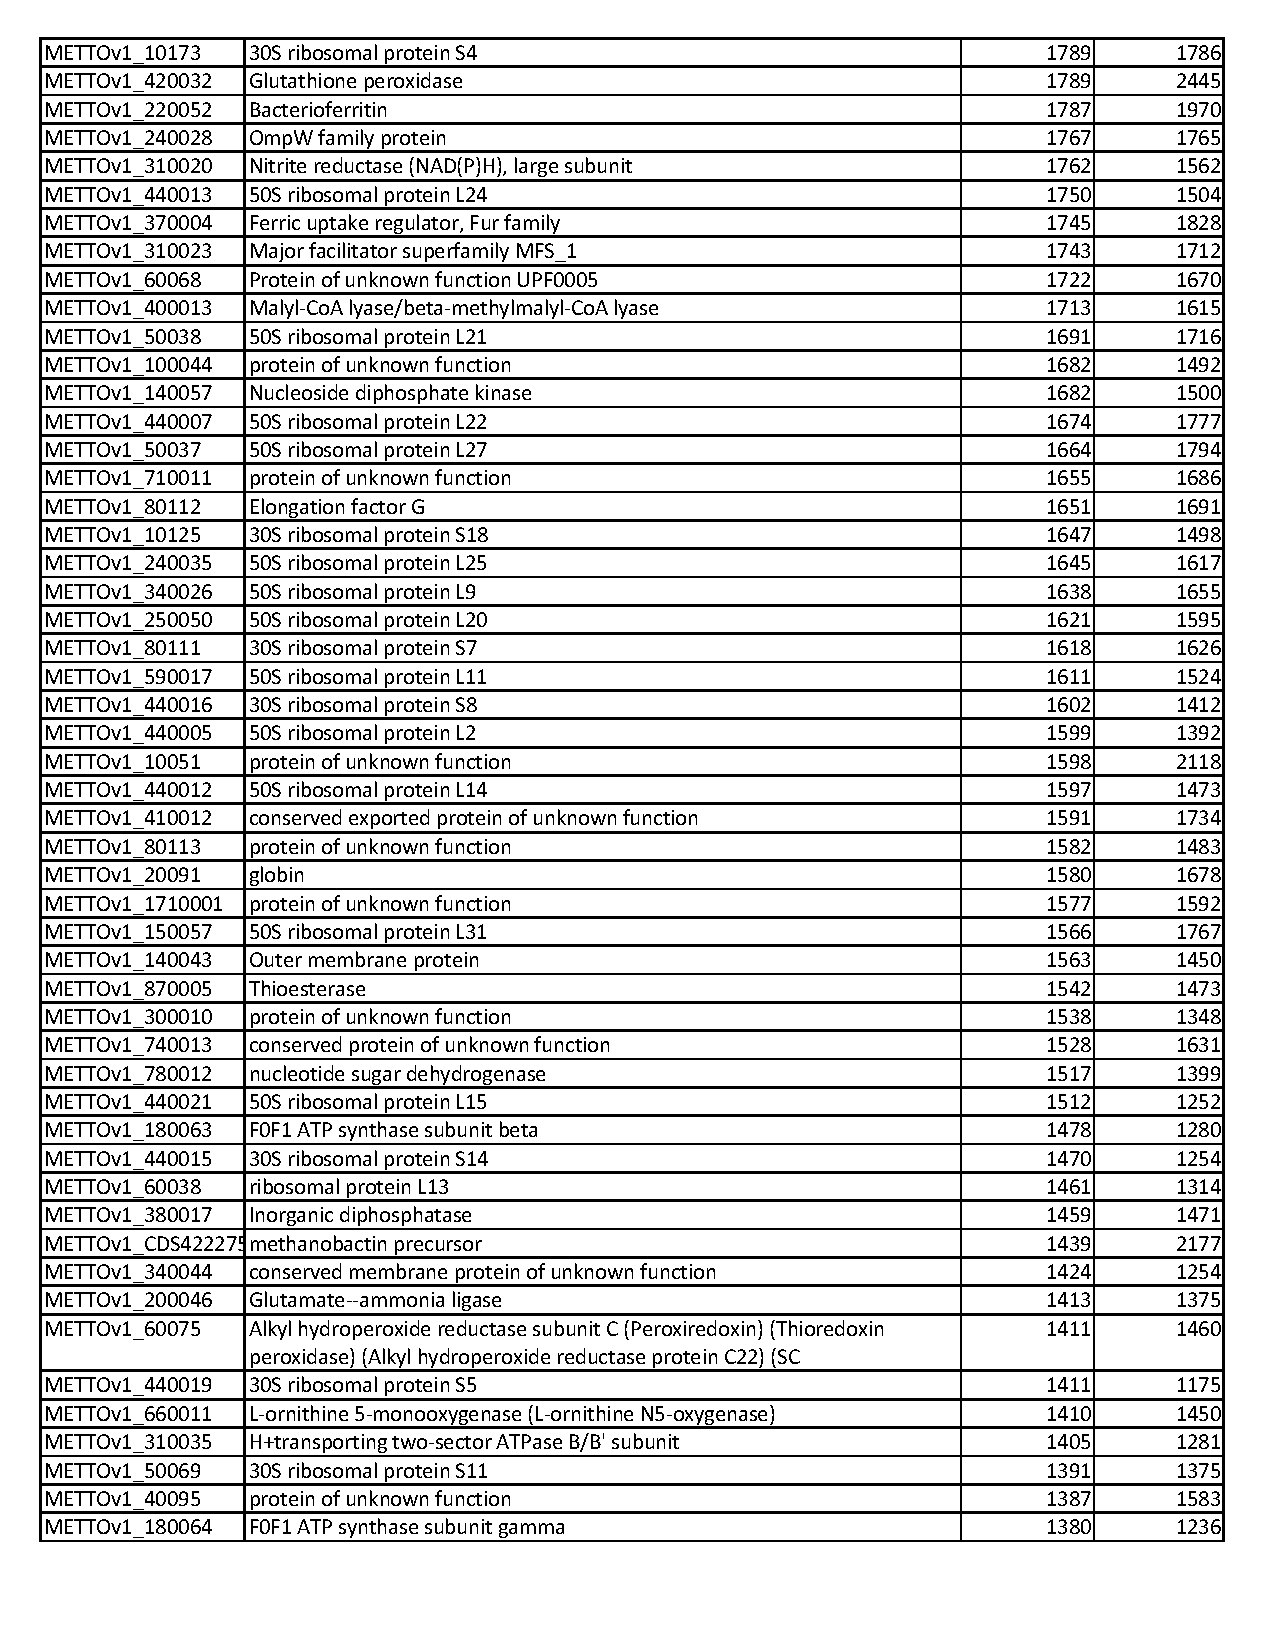
\includegraphics[width=1.0\textwidth]{./tex/chapter1/figures/supplemental/TableS2c.pdf}
\end{figure}
\begin{figure}[H]
\centering
    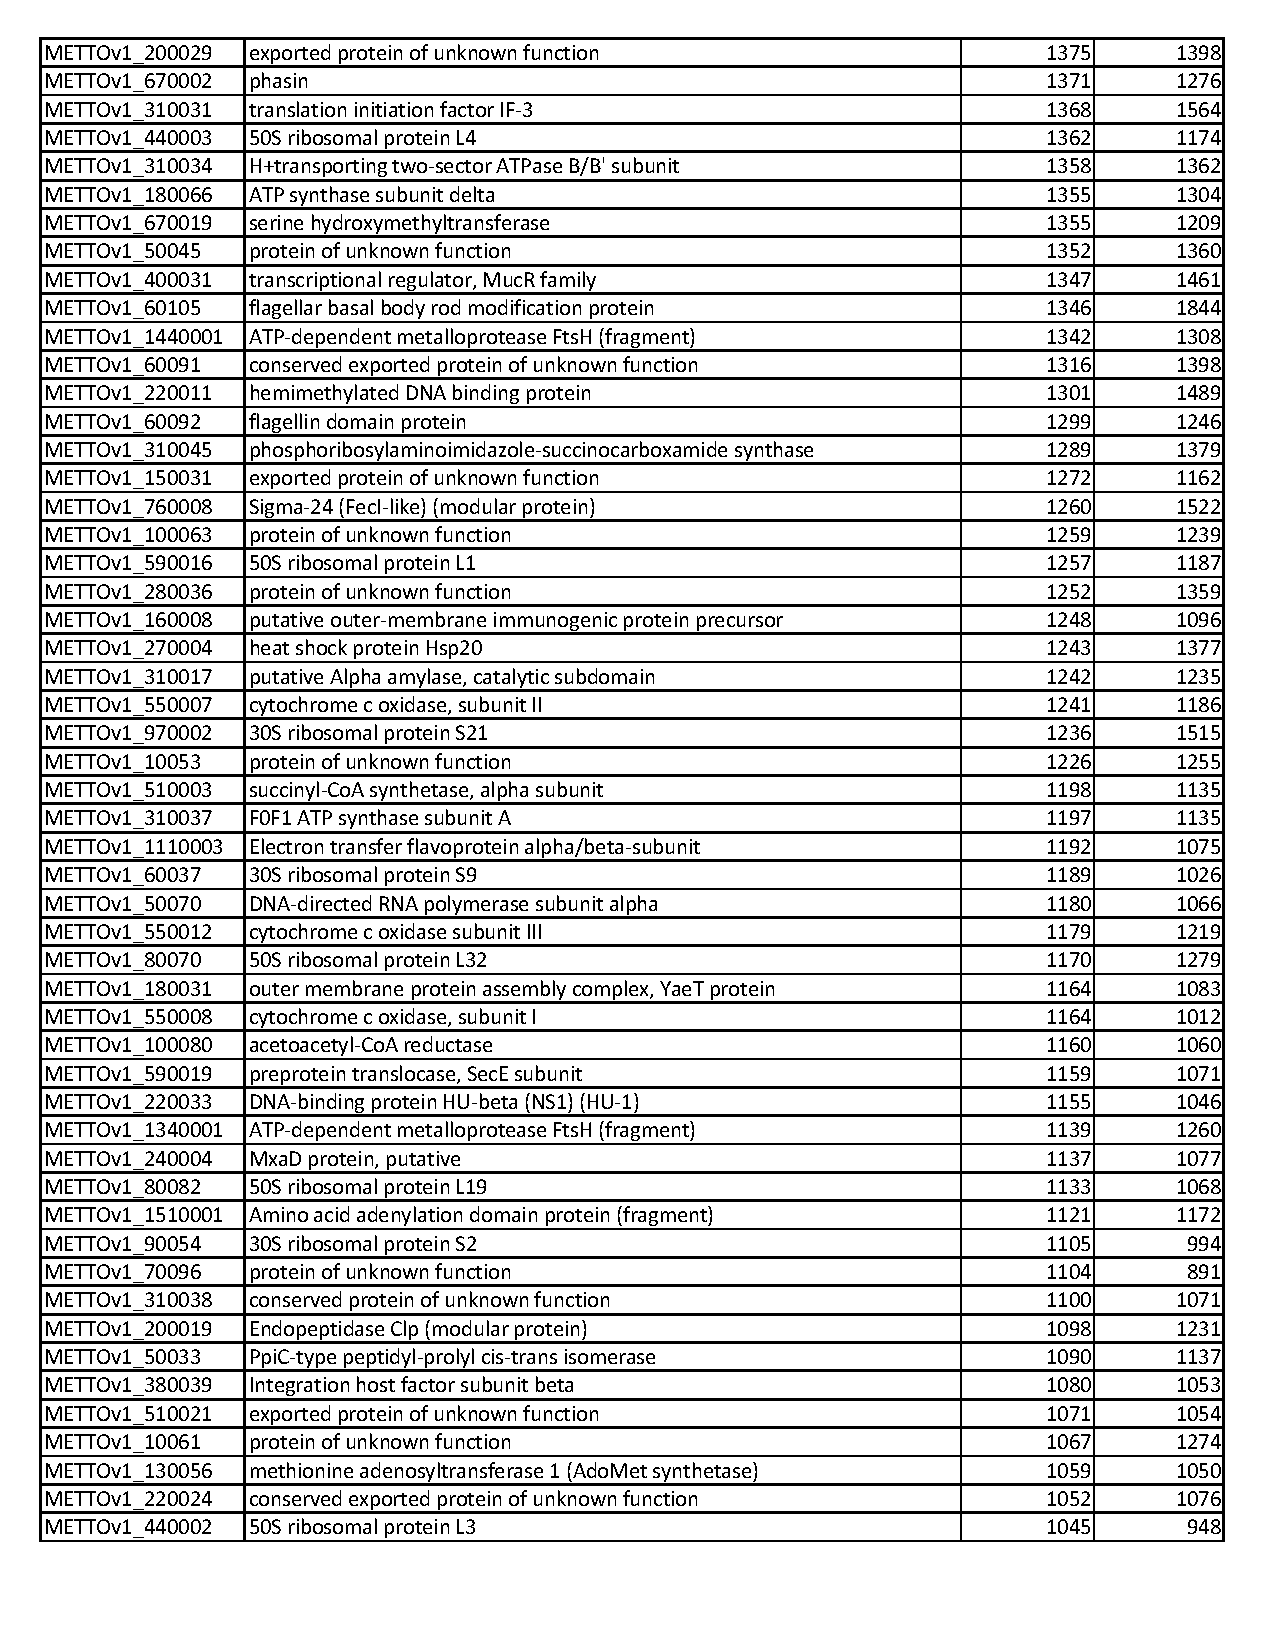
\includegraphics[width=1.0\textwidth]{./tex/chapter1/figures/supplemental/TableS2d.pdf}
\end{figure}


\begin{table}[H]
\caption{Summary of putative transcription site mapping
	%(Note that the published sequences need references added).
	}
\label{table:ChA_S3}
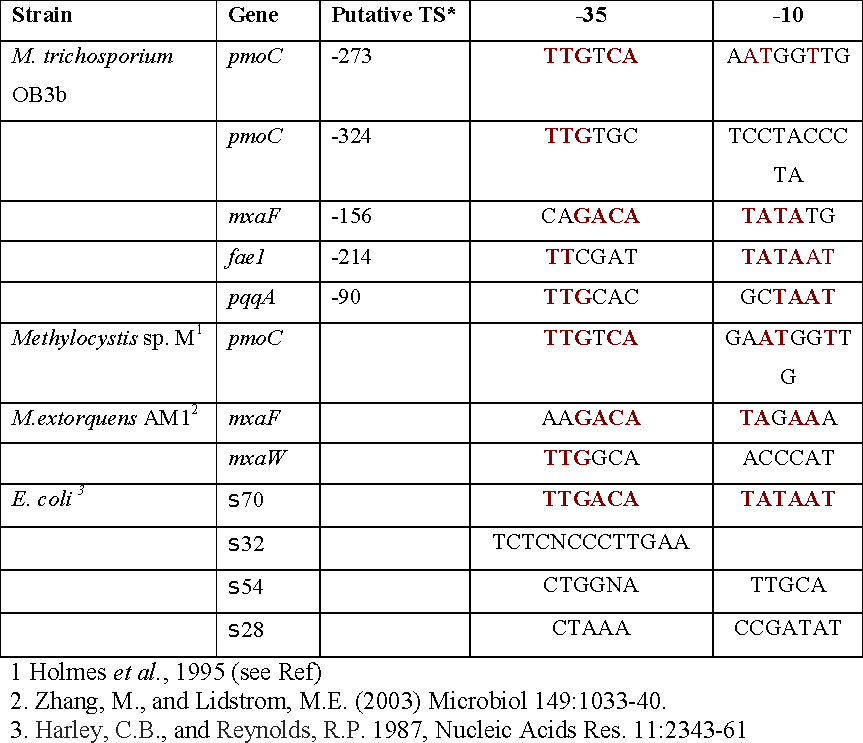
\includegraphics[width=1.0\textwidth]{./tex/chapter1/figures/supplemental/TableS3.pdf}
\end{table}

\begin{table}[H]
\caption{Summary of RNA-seq (Illumina) reads.}
\label{table:ChA_S4}
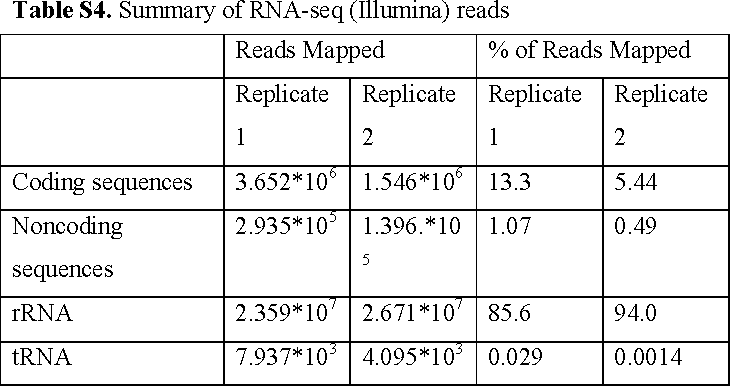
\includegraphics[width=0.8\textwidth]{./tex/chapter1/figures/supplemental/TableS4.pdf}
\end{table}

\begin{table}[H]
\caption{Genes removed from reference scaffold before alignment.}
\label{table:ChA_S5}
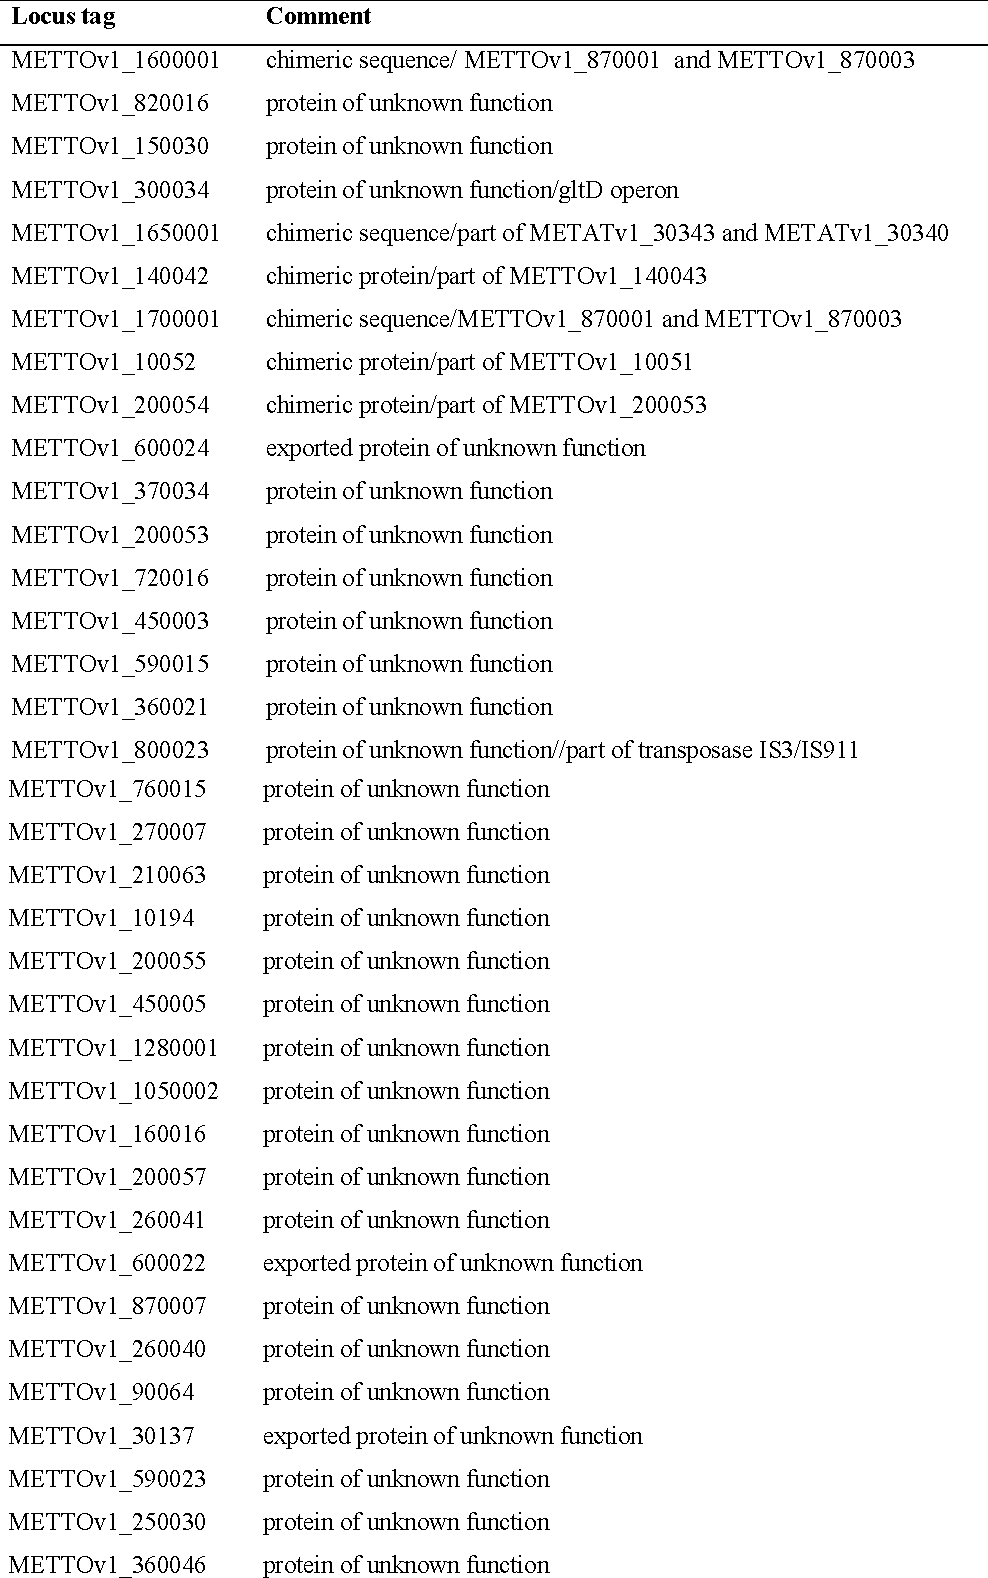
\includegraphics[width=0.75\textwidth]{./tex/chapter1/figures/supplemental/TableS5.pdf}
\end{table}


